\documentclass{estiloDeTesis}
\usepackage{makeidx}
\usepackage{hyperref}
\hypersetup{breaklinks=true,colorlinks=true,linkcolor=black,citecolor=black,urlcolor=black}
\usepackage{pstricks}
\usepackage{url}
\usepackage{doi} 
\usepackage{footnote}
\usepackage{threeparttable}
\usepackage{microtype}
\usepackage[margin=10pt,font=small,labelfont=bf,labelsep=endash]{caption}
\usepackage{natbib}
\usepackage{pdflscape}
\usepackage[section]{placeins}
\usepackage{rotfloat}
\restylefloat{figure}
\floatstyle{boxed} 

%%%%%%%%%%%%%% Footnote format
\usepackage[doublespacing]{setspace}
\usepackage[bottom,hang]{footmisc}

\setlength{\footnotemargin}{-0.5em}
\setlength{\footnotesep}{-0.5em}
%%%%%%%%%%%%%%

\newcommand{\porHacer}[1]{{\color{red}#1}}
\newcommand{\redify}[1]{{\color[RGB]{237,27,35}#1}}
\newcommand{\greenify}[1]{{\color[RGB]{0,166,79}#1}}
\newcommand{\bluefy}[1]{{\color[RGB]{0,157,220}#1}}
\newcommand{\amark}{\multicolumn{1}{c|}{\bluefy{$\approx$}}}%
\newcommand{\cmark}{\multicolumn{1}{c|}{\greenify{\checkmark}}}%
\newcommand{\xmark}{\multicolumn{1}{c|}{\redify{\text{\sffamily X}}}}%

\def\titulo{Por definir}
\def\autor{Iv\'an Alejandro Guerra L\'opez}
\def\matricula{1425688}
\def\fecha{agosto 2014}
\def\asesor{Dra.\ Satu Elisa Schaeffer}
\def\coasesor{Dr. C\'esar Guerra Torres}
\def\revisor{Dr. Romeo S\'anchez Nigenda}
\def\vobo{M.C.\ Arnulfo Trevi\~{n}o Cubero}

\newcommand{\pname}[1]{{\fontfamily{phv}\selectfont{#1}\fontfamily{cmr}\selectfont}}
\setcounter{secnumdepth}{5}
\makeindex

\usepackage{listings}
\usepackage{tikz-uml}
\lstdefinelanguage{tikzuml}{language=[LaTeX]TeX, classoffset=0, morekeywords={umlbasiccomponent, umlprovidedinterface, umlrequiredinterface, umldelegateconnector, umlassemblyconnector, umlVHVassemblyconnector, umlHVHassemblyconnector, umlnote, umlusecase, umlactor, umlinherit, umlassoc, umlVHextend, umlinclude, umlstateinitial, umlbasicstate, umltrans, umlstatefinal, umlVHtrans, umlHVtrans, umldatabase, umlmulti, umlobject, umlfpart, umlcreatecall, umlclass, umlvirt, umlunicompo, umlimport, umlaggreg}, keywordstyle=\color{blue}, classoffset=1, morekeywords={umlcomponent, umlsystem, umlstate, umlseqdiag, umlcall, umlcallself, umlfragment, umlpackage}, keywordstyle=\color{red}, classoffset=0,  sensitive=true, morecomment=[l]{\%}}

\definecolor{rosso}{RGB}{220,57,18}
\definecolor{giallo}{RGB}{255,153,0}
\definecolor{blu}{RGB}{102,140,217}
\definecolor{verde}{RGB}{16,150,24}
\definecolor{viola}{RGB}{153,0,153}

\makeatletter

% Funciones para generar os piecharts
\tikzstyle{chart}=[
    legend label/.style={font={\scriptsize},anchor=west,align=left},
    legend box/.style={rectangle, draw, minimum size=5pt},
    axis/.style={black,semithick,->},
    axis label/.style={anchor=east,font={\tiny}},
]

\tikzstyle{bar chart}=[
    chart,
    bar width/.code={
        \pgfmathparse{##1/2}
        \global\let\bar@w\pgfmathresult
    },
    bar/.style={very thick, draw=white},
    bar label/.style={font={\bf\small},anchor=north},
    bar value/.style={font={\footnotesize}},
    bar width=.75,
]

\tikzstyle{pie chart}=[
    chart,
    slice/.style={line cap=round, line join=round, very thick,draw=white},
    pie title/.style={font={\bf}},
    slice type/.style 2 args={
        ##1/.style={fill=##2},
        values of ##1/.style={}
    }
]

\pgfdeclarelayer{background}
\pgfdeclarelayer{foreground}
\pgfsetlayers{background,main,foreground}


\newcommand{\pie}[3][]{
    \begin{scope}[#1]
    \pgfmathsetmacro{\curA}{90}
    \pgfmathsetmacro{\r}{1}
    \def\c{(0,0)}
    \node[pie title] at (90:1.3) {#2};
    \foreach \v/\s in{#3}{
        \pgfmathsetmacro{\deltaA}{\v/100*360}
        \pgfmathsetmacro{\nextA}{\curA + \deltaA}
        \pgfmathsetmacro{\midA}{(\curA+\nextA)/2}

        \path[slice,\s] \c
            -- +(\curA:\r)
            arc (\curA:\nextA:\r)
            -- cycle;
        \pgfmathsetmacro{\d}{max((\deltaA * -(.5/50) + 1) , .5)}

        \begin{pgfonlayer}{foreground}
        \path \c -- node[pos=\d,pie values,values of \s]{$\v\%$} +(\midA:\r);
        \end{pgfonlayer}

        \global\let\curA\nextA
    }
    \end{scope}
}

\newcommand{\legend}[2][]{
    \begin{scope}[#1]
    \path
        \foreach \n/\s in {#2}
            {
                  ++(0,-10pt) node[\s,legend box] {} +(5pt,0) node[legend label] {\n}
            }
    ;
    \end{scope}
}
%%%%%%%%%%%%%%%%%%%%%%%%%%%

\begin{document}
\frontmatter
\pagestyle{main}
\def\uanl{Universidad Aut\'{o}noma de Nuevo Le\'{o}n}
\def\fime{Facultad de Ingenier\'{\i}a Mec\'{a}nica y El\'{e}ctrica}
\def\depg{Divisi\'{o}n de Estudios de Licenciatura}
\def\snnl{San Nicol\'{a}s de los Garza, Nuevo Le�n}
\thispagestyle{empty}

\begin{scshape}
\begin{center}
	{\Large \uanl} \\[6mm]
	{\large \fime} \\[6mm]
	{\large \depg}
	\vskip 16mm
	
\includegraphics[height=55mm]{uanl}
	\vskip 14mm
	\begin{tabular}{p{11cm}}
		\centering
		{\large \titulo}
	\end{tabular}
	\vskip 8mm
	{por}\\[8mm]
	{\large \autor}\\[8mm]
	{en opci\'{o}n al grado de}\\[3mm]
	{\large Ingeniero en Tecnolog\'{\i}a de Software}
\end{center}

\vfill
\snnl \hfill \fecha
\end{scshape}

\newpage
\thispagestyle{empty}

\begin{scshape}
\begin{center}
	{\Large \uanl} \\[6mm]
	{\large \fime} \\[6mm]
	{\large \depg}
	\vskip 17mm
	
\includegraphics[height=50mm]{fime}
	\vskip 17mm
	\begin{tabular}{p{11cm}}
		\centering
		{\large \titulo}
	\end{tabular}
	\vskip 8mm
	{por}\\[8mm]
	{\large \autor}\\[8mm]
	{en opci\'{o}n al grado de}\\[3mm]
	{\large Ingeniero en Tecnolog\'{\i}a de Software}
\end{center}

\vfill
\snnl \hfill \fecha
\end{scshape}

\newpage
\thispagestyle{empty}
\enlargethispage{5mm}

\begin{center}
{\bf \large \uanl} \\
{\bf \fime} \\
{\bf \depg}
\end{center}
\vskip 5mm

Los miembros del Comit\'{e} de Tesis recomendamos que la
Tesis \guillemotleft \titulo \guillemotright, realizada
por el alumno \autor, con n\'{u}mero de matr�cula \matricula, sea
aceptada para su defensa como opci\'{o}n al grado de Ingeniero en
Tecnolog\'{\i}a de Software.
\vskip 8mm

\begin{center}
El Comit\'{e} de Tesis\\          
\vskip 17mm

\begin{center}
\rule{60mm}{0.3pt}      

\vspace*{-3mm}

\asesor
\vspace*{-4mm}

Asesor
\end{center}

\vspace*{8mm}

\begin{tabular}{cc}
\rule{60mm}{0.3pt} & \rule{60mm}{0.3pt} \\
	\coasesor & \revisor \\
	Revisor & Revisor   \\
\end{tabular}

\vspace*{8mm}

\begin{center}
Vo.\ Bo.\

\vspace*{6mm}

\rule{60mm}{0.3pt}      

\vspace*{-3mm}

\vobo

\vspace*{-3mm}

\depg
\end{center}

\vfill

\snnl, \fecha

\end{center}

\chapter*{Agradecimientos}

Quiero agradecer a las personas que conforman la Facultad de Ingenier\'ia Mec\'anica y El\'ectrica y en general a la Universidad Aut\'onoma de Nuevo Le\'on ya que de alguna manera gracias a ellos estoy aqu\'i. 

Tambi\'en agradezco a todos los profesores que me dieron la ense\~nanza necesaria y el apoyo que busqu\'e durante mis estudios. A mis compa\~neros y amigos que me ayudaron a corregir mis errores y a resolver mis dudas cuando las ten\'ia.

Agradezco profundamente a mi asesora de tesis la {\asesor} por apoyarme en mi trabajo, por todo lo que me ense\~n\'o, por todas las veces que me llam\'o la atenci\'on, por las oportunidades que me dio y en general por formar parte de casi toda mi formaci\'on profesional.

A los miembros del comit\'e de tesis el {\coasesor} y el {\revisor} por sus comentarios y sugerencias en este trabajo.

Agradezco a mis padres V\'ictor Alejandro Briones V\'azquez y Gloria Leticia Segovia S\'aenz porque ellos creyeron en mi a\'un cuando ya no ve\'ia soluci\'on a un problema o cuando cre\'ia que ya no pod\'ia continuar, por inculcarme el estudio cuando era peque\~no, por guiarme por el camino correcto y sobre todo por apoyarme y por estar ah\'i cuando los necesitaba.
\newpage


%Resumen

\chapter*{Resumen}
\markboth{Resumen}{}

\noindent\autor.

\noindent Candidato para el grado de Ingeniero en Tecnolog\'{\i}a de Software.
%\indent 

\noindent\uanl.\\
\noindent\fime.

\noindent T\'{\i}tulo del estudio:

\begin{center}
\begin{tabular}{p{11cm}}
	\centering
	\scshape{\large{\titulo}}
\end{tabular}
\end{center}\bigskip

\noindent N\'{u}mero de p\'{a}ginas: \pageref*{lastpage}.

\paragraph{Objetivos y m\'{e}todo de estudio:}

El objetivo de este trabajo es desarrollar un software que utilice t\'ecnicas de an\'alisis de se\~nales para reconocer ciertos patrones sonoros en la m\'usica, de esta manera generar una lista de reproducci\'on basada en el ritmo obtenido de los archivos reproducidos. Adicionalmente se desea experimentar con efectos de transici\'on entre pistas musicales para dar un efecto de reproducci\'on sin pausa entre pistas que aparentemente tienen un ritmo parecido, diferenciar y detectar el principio y final de una pista, as\'i como el momento \'optimo para realizar la transici\'on entre pistas.

\noindent El desarrollo de software consiste en su mayor parte de an\'alisis de informaci\'on obtenida de archivos de sonido, el sistema trabaja en tiempo real, por lo que todo ocurre mientras se reproduce el sonido. La intenci\'on es conocer la opini\'on de los usuarios en cuanto a eficiencia.

\paragraph{Contribuciones y conclusiones:}

La contribuci\'on principal de este trabajo es la aplicaci\'on de algoritmos de reconocimiento de patrones y t\'ecnicas de an\'alisis de se\~nales en un software para lograr una reproducci\'on musical sin pausas, con la intenci\'on de mejorar la experiencia musical del usuario.

\noindent El programa generado fue probado bajo ciertas circunstancias de software y hardware para obtener un an\'alisis de funcionamiento detallado y que servir\'a para mejorar a futuro.

\noindent Firma del asesor: \rule{78mm}{0.3pt}

\vspace*{-4mm}

\noindent \phantom{Firma del asesor: m} \asesor


\tableofcontents
\listoffigures
\listoftables

\clearpage
\pagestyle{main}
\newpage

\mainmatter
\pagestyle{fime}

\nomenclature{LBC}{Location Based Computing}
\nomenclature{GPS}{Global Positioning System}
\nomenclature{PDA}{Personal Data Assistant}
\nomenclature{SMS}{Short Message Service}
\nomenclature{PC}{Personal Computer}
\nomenclature{IT}{Information Technologies}
\nomenclature{LAN}{Local Area Network}
\nomenclature{RFID}{Radio Frequency Identification}
\nomenclature{GSM}{Groupe Special Mobile}
\nomenclature{AR}{Augmented Reality}
\nomenclature{HCI}{Human-Computer Interaction}
\nomenclature{CV}{Computer Vision}
\nomenclature{VE}{Virtual Environment}
\nomenclature{RGB}{Red Green Blue}
\nomenclature{CRT}{Cathode Ray Tube}
\nomenclature{TM}{Template Matching}
\nomenclature{DG}{Differential Gradient}
\nomenclature{RAM}{Random Access Memory}
\nomenclature{GB}{Giga Byte}
\nomenclature{MHz}{Mega Hertz}
\nomenclature{HTTP}{Hypertext Transfer Protocol}
\nomenclature{P2P}{Peer to Peer}
\nomenclature{SSA}{Shared Situation Awareness}
\nomenclature{IR}{Infrared}
\nomenclature{IrDA}{Infrared Data Association}
\nomenclature{HTTP}{Hypertext Transfer Protocol}
\nomenclature{3G}{3rd Generation}
\nomenclature{3D}{Three-Dimensional Space}
\nomenclature{MP}{Mega Pixel}
\newpage


\chapter{Introducci\'on}
\label{chap:intro}
Desde los primeros a\~{n}os en que el humano fabric\'o y utiliz\'o herramientas, la m\'usica ha formado parte de nuestras vidas, ya sea de forma directa o indirecta siempre habr\'a m\'usica. Inclusive cuando hablamos, a veces sentimos la necesidad de decir frases con cierta entonaci\'on que sigue un ritmo musical. No cabe duda que la m\'usica es importante para nosotros.

\noindent Muchos lo ven como una forma de distraerse del mundo, o como una forma de relajarse. Dependiendo de nuestro estado de \'animo buscaremos ciertos ritmos r\'apidos o lentos, fuertes o suaves, a veces buscando inspiraci\'on o concentraci\'on o simplemente escuchar m\'usica de pasatiempo.
\section{Motivaci\'on}
Desde un punto de vista m\'as t\'ecnico, la m\'usica es una composici\'on de sonidos que en conjunto siguen un ritmo espec\'ifico. Por alguna raz\'on buscamos escuchar sonidos que sigan un ritmo, pero preferimos evitar aquellos sonidos que carecen de el, algo que solemos llamar ruido.

\noindent Dependiendo del gusto de las personas, muchas consideran que ciertos g\'eneros de m\'usica solamente son ruido, mientras que otras los defienden. Los gustos var\'ian de persona a persona, toman influencia en aspectos como la forma en que nos educan, las personas con quien convivimos, las costumbres de la regi\'on, etc\'etera. Estos gustos a veces se ven alterados con el tiempo, factores como cambiar de regi\'on o las modas tambi\'en afectan los gustos.

\noindent Sin importar los g\'eneros musicales, el ruido es algo que perturba lo que escuchamos ya sea porque la calidad de audio es mala, o por los anuncios que alg\'un servicio incluya en su reproductor o simplemente las pausas entre pistas de audio.

\noindent Sabiendo que hay muchas variables que afectan lo que escuchamos, siempre se trata de llegar a un estado de armon�a a\'un sabiendo que cualquier cosa puede interrumpir este estado. ?`C\'omo evitar la interrupci\'on de la sensaci\'on que produce escuchar una pista de sonido? La respuesta es mezclar las pistas de audio en una sola usando la reproducci\'on sin pausas.
\section{Hip\'otesis}
\label{sec:hipo}
Es posible lograr mezclar el inicio y final de dos pistas de audio con ritmo similar mediante el uso de algoritmos de reconocimiento de patrones de tal forma que no se perciba el cambio entre melod\'ias para lograr una reproducci\'on sin pausas.

%Hay que evitar la interrupci\'on de la pista para dar una sensaci\'on de continuidad, pues las personas prefieren escuchar una sola melod\'ia que siga un ritmo sin interrupci\'on a escuchar varias melod\'ias con variaciones en su ritmo.

%Hay que considerar que la reproducci\'on sin pausa no siempre consiste en continuar r\'apidamente una pista despu\'es de al otra, ya que entre pistas de audio hay variaciones de ritmo. Es necesario mezclar los sonidos, es decir, buscar en la parte final de la primera pista y la parte inicial de la segunda un fragmento que sea compatible en ritmo, mezclarlos e iniciar una transici\'on suave para lograr un efecto de pista continua.

\section{Objetivos}
\label{sec:objs}
%La idea de este tipo de mezclado es similar al efecto llamado crossfading, pero se diferencia en que el crossfading mezcla independientemente del ritmo, b\'asicamente empieza una transici\'on suave entre los \'ultimos segundos de la primera pista y los primeros segundos de la segunda.

El objetivo principal es crear una herramienta capaz de reproducir archivos de sonido de forma continua, y mediante un algoritmo mezclar el inicio y final de las pistas reproducidas de forma que conserven su ritmo y no se perciba el cambio de pista.%que sea capaz de analizar patrones de sonido, compararlos entre las pistas y crear una reproducci\'on continua al mezclar los fragmentos entre las pistas mediante una transici\'on. 

\noindent Los objetivos espec\'ificos son:
\begin{itemize}
\item Crear un reproductor de audio que haga uso de esta herramienta para crear una transici\'on casi imperceptible entre pistas.
\item Realizar pruebas con usuarios con la m\'usica de su gusto.
\item Tratar de implementar la herramienta a alguna otra plataforma ya sea en una aplicaci\'on m\'ovil o una aplicaci\'on web.
\end{itemize}

%Esto abre camino a una gran cantidad de aplicaciones que utilicen el mismo principio como:

%\begin{itemize}
%\item Software capaz de crear mezclas de m\'usica de forma inteligente.
%\item Sistemas de predicci\'on, capaces de crear listas de reproducci\'on basado en an\'alisis previos.
%\item Sistemas de b\'usqueda de m\'usica basada en el ritmo.
%\end{itemize}

\section{Estructura de la tesis}

El presente trabajo de tesis est\'a organizado de la siguiente manera:

\noindent En el cap\'itulo \ref{chap:intro} se habla en forma general sobre la intenci\'on de la tesis y se introducen algunos conceptos en la secci\'on de hip\'otesis y objetivos que son utilizados durante la implementaci\'on del proyecto de tesis.

\noindent En el cap\'itulo \ref{chap:antec} se habla de los antecedentes a los temas que se abordan. Se definen conceptos generales y espec\'ificos a los temas {\em procesamiento de se\~nales} y {\em reconocimiento de patrones}.

\noindent En el cap\'itulo \ref{chap:estart} se presentan trabajos que de alguna manera se relacionan con el tema y proyecto de tesis. Los trabajos presentados se dividen en aquellos que investigan sobre la detecci\'on r\'itmica en una pista de sonido y aquellos que implementan alguna herramienta o aplicaci\'on utilizando la misma.

\noindent En el cap\'itulo \ref{chap:sol} se define la metodolog\'ia; se mencionan las herramientas utilizadas y se muestra el desarrollo del trabajo realizado en cuanto a procesamiento de se\~nales y reconocimiento de patrones. Tambi\'en se muestra el dise\~no e implementaci\'on del software, los datos procesados y la forma en que se trabajan los datos.

\noindent En el cap\'itulo \ref{chap:eval} se eval\'ua el desempe\~no del software desarrollado bajo ciertos par\'ametros, se muestran resultados de pruebas con usuarios  y finalmente se tiene una discusi\'on acerca de lo bueno y lo malo de la implementaci\'on y el algoritmo as\'i como del grado de aceptaci\'on por parte de los usuarios hacia el proyecto.

\noindent En el cap\'itulo \ref{chap:conc} se resumen los resultados obtenidos con el proyecto. Tambi\'en se habla sobre las \'areas de oportunidad del mismo y el trabajo a futuro.
\chapter{Antecedentes}
\label{chap:antec}

La frecuencia es la magnitud que mide la cantidad de pulsos que ocurren en un instante de tiempo. Determina la cantidad de latidos del coraz\'on o el {\em tempo}\footnote{El {\em tempo} es la velocidad con la que se ejecuta una pieza musical.} musical; ambos medidos en {\em pulsos por minuto} (bpm, del ingl\'es {\em beats per minute}). Para determinar la frecuencia en una onda es necesario saber cu\'al es su longitud de onda. La longitud de onda se determina por la distancia entre dos {\em crestas}\footnote{La {\em cresta} es el punto m\'as alto de una onda.} o dos {\em valles}\footnote{El {\em valle} es el punto m\'as bajo de una onda.} consecutivos.

\noindent La figura \ref{fig:freq} muestra un ejemplo de gr\'afica de una onda cuya frecuencia disminuye con el progreso del tiempo.

\begin{figure}[h!]
\begin{center}
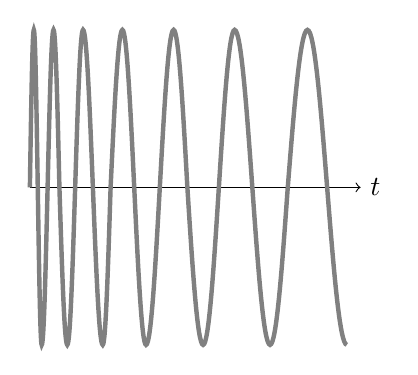
\begin{tikzpicture}
\shorthandoff{<>."}
  \draw[->] (0,0) -- (4.2,0) node[right] {$t$};
  \draw [x=0.5cm,y=2cm, ultra thick, gray] (0,0) 
  sin (0.1,1) cos (0.2,0) sin (0.3,-1) 
  cos (0.45,0) sin (0.6,1) cos (0.75,0) 
  sin (0.95,-1) cos (1.15,0) sin (1.35,1)
  cos (1.6,0) sin (1.85,-1) cos (2.05,0) 
  sin (2.35,1) cos (2.65,0) sin (2.95,-1)
  cos (3.3,0) sin (3.65,1) cos (4,0)
  sin (4.4,-1) cos (4.8,0) sin (5.2,1)
  cos (5.65,0) sin (6.1,-1) cos (6.55,0)
  sin (7.05,1) cos (7.55,0) sin (8.05,-1);
  \shorthandon{<>."}
\end{tikzpicture}
\end{center}
\caption[Frecuencia mayor a menor]{La onda disminuye su frecuencia con la progresi\'on de tiempo $t$.}
\label{fig:freq}
\end{figure}

\noindent \citet{StevenAudio} menciona que el o\'ido humano es un \'organo sumamente complejo. Es sensible a la vibraci\'on de las ondas mec\'anicas producidas a cierta frecuencia. Espec\'ificamente el umbral de audici\'on va desde los 20Hz hasta los 20kHz. El o\'ido es menos sensible a frecuencias m\'as bajas o m\'as altas a las anteriores.

\noindent La {\em c\'oclea} es una estructura interna del o\'ido llena del l\'iquido por el cual viajan las ondas recibidas, solo una porci\'on de las ondas logran pasar y estimulan el nervio auditivo. De esta manera podemos oir.

%\section{Conceptos generales}

\noindent Los sonidos que se reproducen en la computadora o en cualquier otro dispositivo electr\'onico est\'an preparados para el o\'ido humano. Al procesar el sonido se filtran las frecuencias no audibles, de esta manera se ahorra espacio, tambi\'en se procesa el sonido a una velocidad tal que los fragmentos de la pista de sonido no produzcan silencios.

\noindent Generalmente estos fragmentos son almacenados en archivos los cuales son tratados de alguna manera para reproducirlos. Estos archivos contienen informaci\'on b\'asica que indica la forma en que se reproducir\'a el sonido, como el n\'umero de fragmentos de sonido en el archivo o la cantidad de fragmentos que se reproducen por segundo. El archivo tambi\'en contiene los datos del sonido a reproducir comprimidos en alg\'un formato que el reproductor puede interpretar.

\noindent Para reproducir un sonido en alg\'un dispositivo electr\'onico se lleva a cabo una serie de procesos algor\'itmicos que sirven para interpretar los datos almacenados en los archivos, algo conocido como {\em decodificaci\'on}. Una vez decodificados los datos se obtiene informaci\'on que describe una {\em onda ac\'ustica} \cite{izaguirre2008sistemas}.

\noindent Cuando se reproduce un sonido lo que en realidad se escucha es una representaci\'on del sonido real, que ha sido procesada. La onda que se reproduce puede ser muy similar pero no igual al sonido original. Este sonido producido es conocido como {\em sonido digital}.

\section{Procesamiento de se\~nales}

La producci\'on de sonido digital es un proceso de transformaci\'on de una se\~nal anal\'ogica a digital. \citet{Baher} describe tres etapas:

\begin{description}
\item[Muestreo.]{El proceso en el que una se\~nal anal\'ogica es transformada en {\em datos discretizados}.}
\item[Cuantificaci\'on.]{Es la {\em digitalizaci\'on} de los datos obtenidos durante el muestreo de la se\~nal.}
\item[Codificaci\'on.]{El proceso de almacenado de la se\~nal discretizada en alg\'un formato de {\em codec}.}
\end{description}

\noindent Estas tres etapas se discuten en detalle a continuaci\'on.

\subsection{Muestreo}

Para poder trabajar con sonidos digitales, es necesario reducir las se\~nales deben a muestras discretas de un dominio de tiempo discreto. Esta operaci\'on es llamada {\em muestreo}.

\noindent El muestreo consiste en tomar valores de una se\~nal de tiempo continuo en instantes de tiempo m\'ultiplos de $T$, llamado intervalo de muestreo. La cantidad $F_s = 1/T$ es llamada {\em frecuencia de muestreo} \cite{Davide}. En la figura \ref{fig:muest} se ilustra un ejemplo del proceso de muestreo.

\begin{figure}[h!]
\centering
\begin{minipage}[c][5cm][t]{.5\textwidth}
\centering
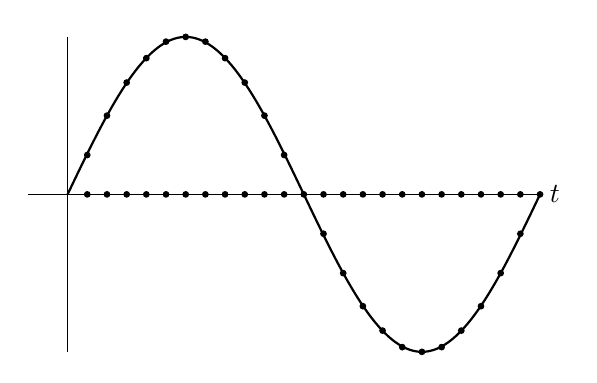
\begin{tikzpicture}
\shorthandoff{<>."}
  \draw[-] (-.5,0) -- (6,0) node[right] {$t$};
  \draw[-] (0,-2) -- (0,2) node[right] {$$};
  \draw [x=0.5cm,y=2cm, thick, black] (0,0) 
  sin (3,1) cos (6,0) sin (9,-1) cos (12,0);  
  \filldraw (0.25,0) circle (1pt);
  \filldraw (0.25,.5) circle (1pt);
  
  \filldraw (0.5,0) circle (1pt);
  \filldraw (0.5,1) circle (1pt);
  
  \filldraw (0.75,0) circle (1pt);
  \filldraw (0.75,1.42) circle (1pt);
  
  \filldraw (1,0) circle (1pt);
  \filldraw (1,1.73) circle (1pt);
    
  \filldraw (1.25,0) circle (1pt);
  \filldraw (1.25,1.94) circle (1pt);

  \filldraw (1.5,0) circle (1pt);
  \filldraw (1.5,2) circle (1pt);
  
  \filldraw (1.75,0) circle (1pt);
  \filldraw (1.75,1.94) circle (1pt);

  \filldraw (2,0) circle (1pt);
  \filldraw (2,1.73) circle (1pt);

  \filldraw (2.25,0) circle (1pt);
  \filldraw (2.25,1.42) circle (1pt);

  \filldraw (2.5,0) circle (1pt);
  \filldraw (2.5,1) circle (1pt);

  \filldraw (2.75,0) circle (1pt);
  \filldraw (2.75,.5) circle (1pt);

  \filldraw (3,0) circle (1pt);

  \filldraw (3.25,0) circle (1pt);
  \filldraw (3.25,-.5) circle (1pt);

  \filldraw (3.5,0) circle (1pt);
  \filldraw (3.5,-1) circle (1pt);

  \filldraw (3.75,0) circle (1pt);
  \filldraw (3.75,-1.42) circle (1pt);

  \filldraw (4,0) circle (1pt);
  \filldraw (4,-1.73) circle (1pt);

  \filldraw (4.25,0) circle (1pt);
  \filldraw (4.25,-1.94) circle (1pt);

  \filldraw (4.5,0) circle (1pt);
  \filldraw (4.5,-2) circle (1pt);

  \filldraw (4.75,0) circle (1pt);
  \filldraw (4.75,-1.94) circle (1pt);

  \filldraw (5,0) circle (1pt);
  \filldraw (5,-1.73) circle (1pt);

  \filldraw (5.25,0) circle (1pt);
  \filldraw (5.25,-1.42) circle (1pt);

  \filldraw (5.5,0) circle (1pt);
  \filldraw (5.5,-1) circle (1pt);

  \filldraw (5.75,0) circle (1pt);
  \filldraw (5.75,-.5) circle (1pt);

  \filldraw (6,0) circle (1pt);
  \shorthandon{<>."}
\end{tikzpicture}

\\a)
\end{minipage}%
\begin{minipage}[c][5cm][t]{.5\textwidth}
\centering
\begin{tikzpicture}
\shorthandoff{<>."}
  \draw[-] (-.5,0) -- (6,0) node[right] {$t$};
  \draw[-] (0,-2) -- (0,2) node[right] {$$};
  \draw (0.25,0) -- (0.25,.5);
  
  \draw (0.5,0) -- (0.5,1);
  
  \draw (0.75,0) -- (0.75,1.42);
  
  \draw (1,0) -- (1,1.73);
    
  \draw (1.25,0) -- (1.25,1.94);

  \draw (1.5,0) -- (1.5,2);
  
  \draw (1.75,0) -- (1.75,1.94);

  \draw (2,0) -- (2,1.73);

  \draw (2.25,0) -- (2.25,1.42);

  \draw (2.5,0) -- (2.5,1);

  \draw (2.75,0) -- (2.75,.5);

  \draw (3.25,0) -- (3.25,-.5);

  \filldraw (3.5,0) -- (3.5,-1);

  \filldraw (3.75,0) -- (3.75,-1.42);

  \filldraw (4,0) -- (4,-1.73);

  \filldraw (4.25,0) -- (4.25,-1.94);

  \filldraw (4.5,0) -- (4.5,-2);

  \filldraw (4.75,0) -- (4.75,-1.94);

  \filldraw (5,0) -- (5,-1.73);

  \filldraw (5.25,0) -- (5.25,-1.42);

  \filldraw (5.5,0) -- (5.5,-1);

  \filldraw (5.75,0) -- (5.75,-.5);

  \shorthandon{<>."}
\end{tikzpicture}

\\b)
\end{minipage}%
\caption[Proceso de muestreo]{En a) se toman muestras de una onda en intervalos de tiempo regulares $t$, en b) se hace una representaci\'on digital de la onda.}
\label{fig:muest}
\end{figure}

\subsection{Cuantificaci\'on}

Los datos obtenidos del muestreo ahora pueden ser representados como una se\~nal de tiempo discreto y valores continuos. Con la cuantificaci\'on los valores se discretizan. El valor de cada muestra es aproximado entonces con un valor de un conjunto finito de posibles valores. La diferencia entre el valor continuo y su aproximaci\'on se le denomina error de cuantificaci\'on \cite{Baher}. En la figura \ref{fig:cuant} se puede ver un ejemplo de cuantificaci\'on de una se\~nal.

\begin{figure}[h!]
\centering
\begin{minipage}[c][5cm][t]{.5\textwidth}
\centering
\begin{tikzpicture}
\shorthandoff{<>."}
  \draw[-] (-.5,0) -- (6,0) node[right] {$t$};
  \draw[-] (0,-2) -- (0,2) node[right] {$$};
  \draw (0.25,0) -- (0.25,.5);
  \draw (0.25,.5) -- (0.5,.5);

  \draw (0.5,.5) -- (0.5,1);
  \draw (0.5,1) -- (0.75,1);

  \draw (0.75,01) -- (0.75,1.42);
  \draw (0.75,1.42) -- (1,1.42);

  \draw (1,1.42) -- (1,1.73);
  \draw (1,1.73) -- (1.25,1.73);

  \draw (1.25,1.73) -- (1.25,1.94);
  \draw (1.25,1.94) -- (1.5,1.94);

  \draw (1.5,1.94) -- (1.5,2);
  \draw (1.5,2) -- (1.75,2);

  \draw (1.75,2) -- (1.75,1.94);
  \draw (1.75,1.94) -- (2,1.94);

  \draw (2,1.94) -- (2,1.73);
  \draw (2,1.73) -- (2.25,1.73);

  \draw (2.25,1.73) -- (2.25,1.42);
  \draw (2.25,1.42) -- (2.5,1.42);

  \draw (2.5,1.42) -- (2.5,1);
  \draw (2.5,1) -- (2.75,1);

  \draw (2.75,1) -- (2.75,.5);
  \draw (2.75,.5) -- (3,.5);

  \draw (3,.5) -- (3,0);
  \draw (3,0) -- (3.25,0);
  
  \draw (3.25,0) -- (3.25,-.5);
  \draw (3.25,-.5) -- (3.5,-.5);

  \draw (3.5,-.5) -- (3.5,-1);
  \draw (3.5,-1) -- (3.75,-1);
  
  \draw (3.75,-1) -- (3.75,-1.42);
  \draw (3.75,-1.42) -- (4,-1.42);
  
  \draw (4,-1.42) -- (4,-1.73);
  \draw (4,-1.73) -- (4.25,-1.73);

  \draw (4.25,-1.73) -- (4.25,-1.94);
  \draw (4.25,-1.94) -- (4.5,-1.94);

  \draw (4.5,-1.94) -- (4.5,-2);
  \draw (4.5,-2) -- (4.75,-2);

  \draw (4.75,-2) -- (4.75,-1.94);
  \draw (4.75,-1.94) -- (5,-1.94);

  \draw (5,-1.94) -- (5,-1.73);
  \draw (5,-1.73) -- (5.25,-1.73);

  \draw (5.25,-1.73) -- (5.25,-1.42);
  \draw (5.25,-1.42) -- (5.5,-1.42);

  \draw (5.5,-1.42) -- (5.5,-1);
  \draw (5.5,-1) -- (5.75,-1);

  \draw (5.75,-1) -- (5.75,-.5);
  \draw (5.75,-.5) -- (6,-.5);

  \draw (6,-.5) -- (6,0);

  \shorthandon{<>."}
\end{tikzpicture}

\\a)
\end{minipage}%
\begin{minipage}[c][5cm][t]{.5\textwidth}
\centering
\begin{tikzpicture}
\shorthandoff{<>."}
  \draw[-] (-.5,0) -- (6,0) node[right] {$t$};
  \draw[-] (0,-2) -- (0,2) node[right] {$$};
  \draw (0,0) -- (0.25,.5);
  \draw (0.25,.5) -- (0.5,1);

  \draw (0.5,1) -- (0.75,1.42);
  \draw (0.75,1.42) -- (1,1.73);

  \draw (1,1.73) -- (1.25,1.93);

  \draw (1.25,1.94) -- (1.5,2);

  \draw (1.5,2) -- (1.75,1.94);

  \draw (1.75,1.94) -- (2,1.73);

  \draw (2,1.73) -- (2.25,1.42);

  \draw (2.25,1.42) -- (2.5,1);

  \draw (2.5,1) -- (2.75,.5);

  \draw (2.75,.5) -- (3,0);

  \draw (3,0) -- (3.25,-.5);
  
  \draw (3.25,-.5) -- (3.5,-1);

  \draw (3.5,-1) -- (3.75,-1.42);
  
  \draw (3.75,-1.42) -- (4,-1.73);
  
  \draw (4,-1.73) -- (4.25,-1.94);

  \draw (4.25,-1.94) -- (4.5,-2);

  \draw (4.5,-2) -- (4.75,-1.94);

  \draw (4.75,-1.94) -- (5,-1.73);

  \draw (5,-1.73) -- (5.25,-1.42);

  \draw (5.25,-1.42) -- (5.5,-1);

  \draw (5.5,-1) -- (5.75,-.5);

  \draw (5.75,-.5) -- (6,0);

  \shorthandon{<>."}
\end{tikzpicture}

\\b)
\end{minipage}%
\caption[Proceso de cuantificaci\'on]{La representaci\'on digital es discretizada en a) y posteriormente se suavizan los valores de \'esta en b) para dar una forma parecida a la onda original.}
\label{fig:cuant}
\end{figure}

\subsection{Codificaci\'on}

Despu\'es de la cuantificaci\'on se tiene una se\~nal de timepo discreto con valores discretos como la de la figura \ref{fig:cod1} que se puede almacenar en un {\em contenedor}; este contenedor comprime la informaci\'on mediante alg\'un algoritmo de codificaci\'on, puede ser con o sin p\'erdida. La compresi\'on con p\'erdida usa algoritmos que almacenan una se\~nal similar pero no igual a la original. La compresi\'on sin p\'erdida usa un algoritmo que almacena los datos originales, generalmente ocupan una cantidad de espacio en disco mayor \cite{StevenAudio}.

\begin{figure}[h!]
\begin{center}
\scalebox{1.6}{
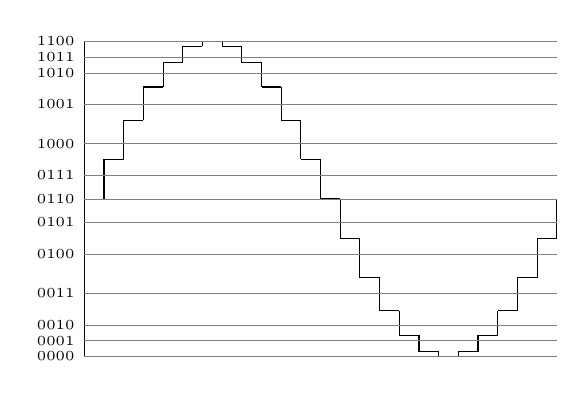
\begin{tikzpicture}
\shorthandoff{<>."}
  \draw[-] (0,-2) -- (0,2) node[right] {$$};
  \draw (0.25,0) -- (0.25,.5);
  \draw (0.25,.5) -- (0.5,.5);

  \draw (0.5,.5) -- (0.5,1);
  \draw (0.5,1) -- (0.75,1);

  \draw (0.75,01) -- (0.75,1.42);
  \draw (0.75,1.42) -- (1,1.42);

  \draw (1,1.42) -- (1,1.73);
  \draw (1,1.73) -- (1.25,1.73);

  \draw (1.25,1.73) -- (1.25,1.94);
  \draw (1.25,1.94) -- (1.5,1.94);

  \draw (1.5,1.94) -- (1.5,2);
  \draw (1.5,2) -- (1.75,2);

  \draw (1.75,2) -- (1.75,1.94);
  \draw (1.75,1.94) -- (2,1.94);

  \draw (2,1.94) -- (2,1.73);
  \draw (2,1.73) -- (2.25,1.73);

  \draw (2.25,1.73) -- (2.25,1.42);
  \draw (2.25,1.42) -- (2.5,1.42);

  \draw (2.5,1.42) -- (2.5,1);
  \draw (2.5,1) -- (2.75,1);

  \draw (2.75,1) -- (2.75,.5);
  \draw (2.75,.5) -- (3,.5);

  \draw (3,.5) -- (3,0);
  \draw (3,0) -- (3.25,0);
  
  \draw (3.25,0) -- (3.25,-.5);
  \draw (3.25,-.5) -- (3.5,-.5);

  \draw (3.5,-.5) -- (3.5,-1);
  \draw (3.5,-1) -- (3.75,-1);
  
  \draw (3.75,-1) -- (3.75,-1.42);
  \draw (3.75,-1.42) -- (4,-1.42);
  
  \draw (4,-1.42) -- (4,-1.73);
  \draw (4,-1.73) -- (4.25,-1.73);

  \draw (4.25,-1.73) -- (4.25,-1.94);
  \draw (4.25,-1.94) -- (4.5,-1.94);

  \draw (4.5,-1.94) -- (4.5,-2);
  \draw (4.5,-2) -- (4.75,-2);

  \draw (4.75,-2) -- (4.75,-1.94);
  \draw (4.75,-1.94) -- (5,-1.94);

  \draw (5,-1.94) -- (5,-1.73);
  \draw (5,-1.73) -- (5.25,-1.73);

  \draw (5.25,-1.73) -- (5.25,-1.42);
  \draw (5.25,-1.42) -- (5.5,-1.42);

  \draw (5.5,-1.42) -- (5.5,-1);
  \draw (5.5,-1) -- (5.75,-1);

  \draw (5.75,-1) -- (5.75,-.5);
  \draw (5.75,-.5) -- (6,-.5);

  \draw (6,-.5) -- (6,0);

\node[left] at (0,-2)	{\tiny 0000};
\node[left] at (0,-1.8)	{\tiny 0001};
\node[left] at (0,-1.6)	{\tiny 0010};
\node[left] at (0,-1.2)	{\tiny 0011};
\node[left] at (0,-.7)	{\tiny 0100};
\node[left] at (0,-.3)	{\tiny 0101};
\node[left] at (0,0)	{\tiny 0110};
\node[left] at (0,.3)	{\tiny 0111};
\node[left] at (0,.7)	{\tiny 1000};
\node[left] at (0,1.2)	{\tiny 1001};
\node[left] at (0,1.6)	{\tiny 1010};
\node[left] at (0,1.8)	{\tiny 1011};
\node[left] at (0,2)	{\tiny 1100};

\draw[-,gray,very thin] (0,2) -- (6,2);
\draw[-,gray,very thin] (0,1.8) -- (6,1.8);
\draw[-,gray,very thin] (0,1.6) -- (6,1.6);
\draw[-,gray,very thin] (0,1.2) -- (6,1.2);
\draw[-,gray,very thin] (0,.7) -- (6,.7);
\draw[-,gray,very thin] (0,.3) -- (6,.3);
\draw[-,gray,very thin] (0,0) -- (6,0);
\draw[-,gray,very thin] (0,-.3) -- (6,-.3);
\draw[-,gray,very thin] (0,-.7) -- (6,-.7);
\draw[-,gray,very thin] (0,-1.2) -- (6,-1.2);
\draw[-,gray,very thin] (0,-1.6) -- (6,-1.6);
\draw[-,gray,very thin] (0,-1.8) -- (6,-1.8);
\draw[-,gray,very thin] (0,-2) -- (6,-2);



  \shorthandon{<>."}
\end{tikzpicture}
}
\end{center}
\caption[Representaci\'on de una se\~nal cuantificada]{La se\~nal cuantificada puede representarse en forma de datos discretizados.}
\label{fig:cod1}
\end{figure}


\noindent Independientemente del metodo de compresi\'on, con la codificaci\'on se obtiene la informaci\'on de la se\~nal en un formato binario como se muestra en la figura \ref{fig:cod}.

\begin{figure}[h!]
\begin{center}
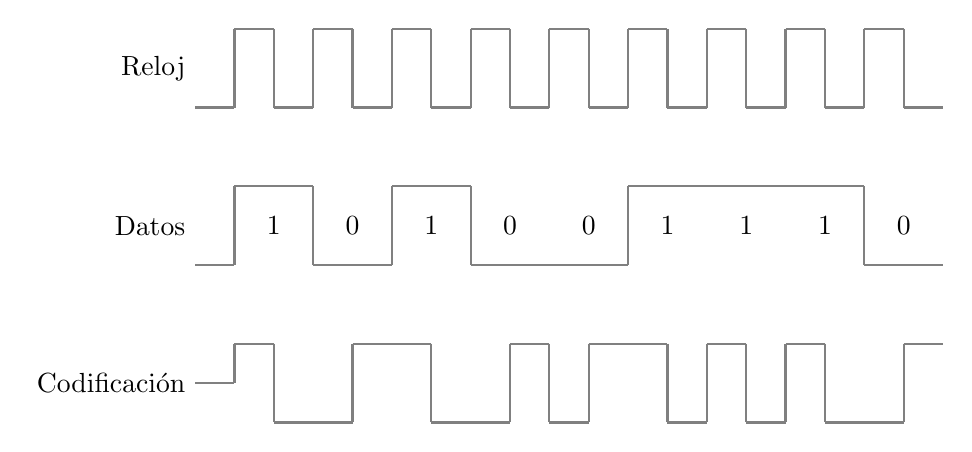
\begin{tikzpicture}
\shorthandoff{<>."}
\draw[thick,gray] (0,2) -- (0.5,2);
\draw[thick,gray] (0.5,2) -- (0.5,3);
\draw[thick,gray] (0.5,3) -- (1,3);
\draw[thick,gray] (1,3) -- (1,2);
\draw[thick,gray] (1,2) -- (1.5,2);
\draw[thick,gray] (1.5,2) -- (1.5,3);
\draw[thick,gray] (1.5,3) -- (2,3);
\draw[thick,gray] (2,3) -- (2,2);
\draw[thick,gray] (2,2) -- (2.5,2);
\draw[thick,gray] (2.5,2) -- (2.5,3);
\draw[thick,gray] (2.5,3) -- (3,3);
\draw[thick,gray] (3,3) -- (3,2);
\draw[thick,gray] (3,2) -- (3.5,2);
\draw[thick,gray] (3.5,2) -- (3.5,3);
\draw[thick,gray] (3.5,3) -- (4,3);
\draw[thick,gray] (4,3) -- (4,2);
\draw[thick,gray] (4,2) -- (4.5,2);
\draw[thick,gray] (4.5,2) -- (4.5,3);
\draw[thick,gray] (4.5,3) -- (5,3);
\draw[thick,gray] (5,3) -- (5,2);
\draw[thick,gray] (5,2) -- (5.5,2);
\draw[thick,gray] (5.5,2) -- (5.5,3);
\draw[thick,gray] (5.5,3) -- (6,3);
\draw[thick,gray] (6,3) -- (6,2);
\draw[thick,gray] (6,2) -- (6.5,2);
\draw[thick,gray] (6.5,2) -- (6.5,3);
\draw[thick,gray] (6.5,3) -- (7,3);
\draw[thick,gray] (7,3) -- (7,2);
\draw[thick,gray] (7,2) -- (7.5,2);
\draw[thick,gray] (7.5,2) -- (7.5,3);
\draw[thick,gray] (7.5,3) -- (8,3);
\draw[thick,gray] (8,3) -- (8,2);
\draw[thick,gray] (8,2) -- (8.5,2);
\draw[thick,gray] (8.5,2) -- (8.5,3);
\draw[thick,gray] (8.5,3) -- (9,3);
\draw[thick,gray] (9,3) -- (9,2);
\draw[thick,gray] (9,2) -- (9.5,2);

\node[left] at (0,2.5){Reloj};

\draw[thick,gray] (0,0) -- (0.5,0);
\draw[thick,gray] (0.5,0) -- (0.5,1);
\draw[thick,gray] (0.5,1) -- (1.5,1);
\draw[thick,gray] (1.5,1) -- (1.5,0);
\draw[thick,gray] (1.5,0) -- (2.5,0);
\draw[thick,gray] (2.5,0) -- (2.5,1);
\draw[thick,gray] (2.5,1) -- (3.5,1);
\draw[thick,gray] (3.5,1) -- (3.5,0);
\draw[thick,gray] (3.5,0) -- (5.5,0);
\draw[thick,gray] (5.5,0) -- (5.5,1);
\draw[thick,gray] (5.5,1) -- (8.5,1);
\draw[thick,gray] (8.5,1) -- (8.5,0);
\draw[thick,gray] (8.5,0) -- (9.5,0);

\node[left] at (0,0.5){Datos};
\node at (1,.5){1};
\node at (2,.5){0};
\node at (3,.5){1};
\node at (4,.5){0};
\node at (5,.5){0};
\node at (6,.5){1};
\node at (7,.5){1};
\node at (8,.5){1};
\node at (9,.5){0};

\draw[thick,gray] (0,-1.5) -- (0.5,-1.5);
\draw[thick,gray] (0.5,-1.5) -- (0.5,-1);
\draw[thick,gray] (0.5,-1) -- (1,-1);
\draw[thick,gray] (1,-1) -- (1,-2);
\draw[thick,gray] (1,-2) -- (2,-2);
\draw[thick,gray] (2,-2) -- (2,-1);
\draw[thick,gray] (2,-1) -- (3,-1);
\draw[thick,gray] (3,-1) -- (3,-2);
\draw[thick,gray] (3,-2) -- (4,-2);
\draw[thick,gray] (4,-2) -- (4,-1);
\draw[thick,gray] (4,-1) -- (4.5,-1);
\draw[thick,gray] (4.5,-1) -- (4.5,-2);
\draw[thick,gray] (4.5,-2) -- (5,-2);
\draw[thick,gray] (5,-2) -- (5,-1);
\draw[thick,gray] (5,-1) -- (6,-1);
\draw[thick,gray] (6,-1) -- (6,-2);
\draw[thick,gray] (6,-2) -- (6.5,-2);
\draw[thick,gray] (6.5,-2) -- (6.5,-1);
\draw[thick,gray] (6.5,-1) -- (7,-1);
\draw[thick,gray] (7,-1) -- (7,-2);
\draw[thick,gray] (7,-2) -- (7.5,-2);
\draw[thick,gray] (7.5,-2) -- (7.5,-1);
\draw[thick,gray] (7.5,-1) -- (8,-1);
\draw[thick,gray] (8,-1) -- (8,-2);
\draw[thick,gray] (8,-2) -- (9,-2);
\draw[thick,gray] (9,-2) -- (9,-1);
\draw[thick,gray] (9,-1) -- (9.5,-1);

\node[left] at (0,-1.5){Codificaci\'on};

\shorthandon{<>."}
\end{tikzpicture}
\end{center}
\caption[Proceso de codificaci\'on]{Proceso de codificaci\'on de una se\~nal transformada a datos.}
\label{fig:cod}
\end{figure}
\section {Transformada r\'apida de Fourier}

Durante el procesamiento de se\~nales puede ser de utilidad analizar frecuencias por separado. La {\em transformada r\'apida de Fourier} permite separar una se\~nal de onda en sus diferentes frecuencias. La figura \ref{fig:trans} muestra un ejemplo gr\'afico del funcionamiento del algoritmo.

\newcommand{\waves}[5][purple]{
\def\a{1+#3}
\def\b{#3}
\def\c{1-#3}
\def\x{#4}
\def\y{#5}
\foreach \val in {0,#3,...,#2}{
\def\i{\x+\val*4}
\def\var{\y+\val}
\draw[ultra thick, #1] (\i + \b*5,-1+\var) cos (\i + \b*4,0+\var); 
\draw[ultra thick, #1] (\i + \b*4,0+\var) sin (\i + \b*3,\a+\var); 
\draw[ultra thick, #1] (\i + \b*3,\a+\var) cos (\i + \b*2,\b+\var); 
\draw[ultra thick, #1] (\i + \b*2,\b+\var) sin (\i + \b,-\c+\var);}
}
\begin{figure}[h!]
\begin{center}
\scalebox{0.6}{
\begin{tikzpicture}
\waves[green]{1}{0.3}{-6}{3}
\waves[blue]{1}{0.2}{-4}{2}
\waves{1}{0.05}{-2}{1}
\waves{1}{0.05}{0}{0}
\waves[blue]{1}{0.2}{2}{-1}
\waves[green]{1}{0.3}{4}{-2}
\draw(-7, 1.5)--(4,-4);
\draw(4,-4)--(10,-2.5);

\node[right] at (4.5,-5){
\includegraphics[height=35mm]{./Figuras/noise}};
\node[right] at (-10,-3.5){
\includegraphics[height=50mm]{./Figuras/freq}};

\end{tikzpicture}}
\end{center}
\caption[Transformada de Fourier]{Comparaci\'on entre una se\~nal y sus frecuencias separadas en ondas individuales.}
\label{fig:trans}
\end{figure}

\noindent A continuaci\'on se describe uno de los algoritmos m\'as usados \cite{walker1996fast}. Se asume que $N = 2^R$ donde $R$ es un entero positivo:
\begin{equation}
H_{k} = \sum_{j=0}^{N-1}h_{j}W^{jk}, \text{donde } W = e^{\pm \frac{2\pi i}{N}}\
\end{equation}

\section{Reconocimiento de patrones}

El reconocimiento de patrones consiste en la extracci\'on de caracter\'isticas importantes en imagenes, sonidos, cadenas de ADN, etc\'etera. \citet{Satosi} menciona que un patr\'on es una entidad, vagamente definida, la cual puede nombrarse.

\noindent \citet{Kittler} en sus notas de seminario menciona que es posible modelar un sistema de tres estados basado en el sistema perceptual de un ser humano:

\begin{description}
\item [Adquisici\'on de datos.] {Consiste en recolectar informaci\'on de alg\'un medio ya sea una c\'amara, un micr\'ofono, o cualquier sensor que genere datos en bruto.}
\item [Extracci\'on de caracter\'isticas.] {Mediante el uso de algoritmos tratar de encontrar informaci\'on relevante dentro de los datos adquiridos.}
\item [Toma de desiciones.] {Cuando se tienen las caracter\'isticas relevantes ahora se clasifican dependiendo del prop\'osito del programa.}
\end{description}

\noindent Existen diferentes aproximaciones a este problema, a continuaci\'on se describen brevemente alg\'unas de la m\'as utilizadas \cite{Anil}.

\begin{description}

\item[Comparaci\'on de plantillas]{Este es el modelo m\'as sencillo y quiz\'a uno de los primeros en existir. Consiste en comparar una plantilla con la informaci\'on de una muestra obtenida buscando similitudes}
\item[Modelo estad\'istico]{Este modelo se basa en la teor\'ia de probabilidad y estad\'istica y supone que se tiene un conjunto de medidas num\'ericas con distribuciones de probabilidad conocidas y a partir de ellas se realiza el reconocimiento.}
\item[Modelo sint\'actico]{Este modelo se basa en encontrar las relaciones estructurales que guardan los objetos de estudio, utilizando la teor\'ia de lenguajes formales. El objetivo es construir una gram\'atica que describa la estructura del universo de objetos.}
\item[Redes neuronales]{Este modelo supone que tiene una estructura de neuronas interconectadas que se estimulan unas a otras, las cuales pueden ser ``entrenadas'' para dar una cierta respuesta cuando se le presentan determinados valores.}

\end{description}
\chapter{Estado del arte}
\label{chap:estart}
Desde hace tiempo se ha investigado en el \'area de reconocimiento de patrones ya sea en imagen o audio, y durante los \'ultimos a\~nos se han desarrollado tecnolog\'ias que la aprovechan, como c\'amaras con detecci\'on de rostros o asistentes personales con procesamiento de lenguaje natural. Cualquier aplicaci\'on de \'esta en la tecnolog\'ia se basa en el mismo principio, buscar caracter\'isticas de inter\'es y procesarlas hasta que pueda ser clasificada.

\section{Revisi\'on de trabajos relacionados}
En cuanto a se\~nales de audio, siempre se trata de buscar aspectos de la onda que sean comunes como por ejemplo tratar de encontrar repeticiones en la pista. Cuando se habla de reconocimiento de patrones sonoros en pistas musicales significa procesar una o varias se\~nales tratando de visualizar zonas en la pista que sean de inter\'es, como las frecuencias de los bajos o de las percusiones que generalmente describen el tempo. 
\subsection{Detecci\'on de tempo}
Gran parte del proyecto que se aborda consiste en realizar b\'usqueda de aspectos r\'itmicos como el tempo, con los que se pretende hacer comparaciones entre pistas y estimar posiciones de tiempo que sean similares entre \'estas.

\noindent Un ejemplo es el de \citet{beatTrack}; en su trabajo presentan un algoritmo de estimaci\'on de tempo y seguimiento r\'itmico mediante la separaci\'on percusivo/arm\'onica de la se\~nal de audio para filtrar caracter\'isticas de cada componente de la pista. La estimaci\'on r\'itmica se logra a partir de los picos tomados de la respuesta de un resonador con los cuales se hace una predicci\'on de ritmo con la cual se deduce la pulsaci\'on.

\noindent Una forma de detectar el tempo es mediante la b\'usqueda de repeticiones r\'itmicas donde \citet{quadMusic} presentan sus matrices de autosimilitud, las cuales son \'utiles para encontrar patrones semejantes y contrastantes en una melod\'ia. Las matrices son creadas por caracter\'isticas extraidas de piezas musicales a varias escalas de tiempo para representar la notaci\'on musical. Postulan que el peso \'optimo de los componentes de la anotaci\'on pueden indicar caracter\'isticas que puedan ser candidatas en una anotaci\'on musical real.

\noindent \citet{swingBeat} propone m\'etodos de estimaci\'on de tempo como el an\'alisis transitorio el cual consiste en analizar por separado segmentos de frecuencias cuando incrementan de forma brusca, esto con la finalidad de detectar percusiones o bajos, o bien detectar cambios r\'apidos de espectro en la se\~nal. Todo esto suponiendo que se trata de una pista con un ritmo constante.

\noindent Por otra parte \citet{perceptTempo} presentan el problema del reconocimiento de tempo como un problema de clasificaci\'on estad\'istica. Definen cuatro clases de tempo basadas en la percepci\'on humana y no en detecci\'on de repetici\'ones pues no descubren el ritmo como tal. Sus clases se definen como: muy lentos, lentos, r\'apidos y muy r\'apidos, dependiendo de la cantidad de pulsos por minuto en una pista. Clasifican el tempo de un sonido usando se\~nales monof\'onicas analizadas en ventanas de tiempo de 30 milisegundos y despu\'es combin\'andolas en grupos de cuatro fragmentos. Un vector final de 128 elementos que consiste en el promedio y varianza de cada grupo es analizado para su posterior clasificaci\'on.

\noindent \citet{tempoMP3} proponen un sistema de detecci\'on de tempo distinto a lo general exclusivo para archivos en formato MP3\footnote{MPEG-2 Audio Layer III o MP3 es un formato de audio com\'un usado para m\'usica tanto en computadoras como en reproductores de audio.} \cite{rfc3003} ya que se basa en la caracter\'istica de \'estos en almacenar cambios en forma de {\em transformadas de coseno}\footnote{La {\em transformada discreta de coseno} es una transformada basada en la transformada de Fourier discreta, pero utilizando �nicamente n�meros reales.} discretas modificadas. \'Esta utiliza un patron de cambio de ventana que hace referencia a cambios en la onda y se encuentra alineada con la tabla de percusiones. No hay an\'alisis de frecuencia, sino que utilizan el patron obtenido de esta l\'inea y un {\em metr\'onomo}.

\noindent Otro sistema propuesto es el de \citet{realtimeTempo} quien realiza un an\'alisis de autocorrelaci\'on envolvente para una se\~nal con la que despu\'es crea una funci\'on ponderada basada en la autocorrelaci\'on para estimar el tempo de una pista. Todo calculado por las amplitudes pico y las posiciones de la autocorrelaci\'on en tiempo real. Con ello se estima una aproximaci\'on de lo que un humano escucha e interpreta como ritmo en una pista.

\noindent Por \'ultimo se menciona el trabajo de \citet{rhythmRep} quienes utilizan algoritmos de an\'alisis de informaci\'on de tempo y almacenamiento en bases de datos via aprendizaje autom\'atico. Ellos incluyen informaci\'on conocida de los ritmos existentes para aumentar el desempe\~no de sus algoritmos. A su finalizaci\'on comparan los resultados con una base de datos musical. Al descomponer una pieza en varios fragmentos hacen una evaluaci\'on utilizando informaci\'on existente sobre el ritmo comparando y tratando de acertar tiempos en los que hay picos en la onda. Todo funciona como un {\em mecanismo no supervisado}\footnote{El {\em aprendizaje no supervisado} es un m�todo de aprendizaje autom\'atico donde un modelo es ajustado a las observaciones. Se distingue del aprendizaje supervisado por el hecho de que no hay un conocimiento a priori.} que busca patrones espectrales en las frecuencias que coincidan con la informaci\'on proporcionada.

\subsection{Aplicaciones con el tempo}

Una vez que se tiene la informaci\'on de un tempo aproximado, se puede buscar caracter\'isticas en los sonidos que nos permiten generar aplicaciones de todo tipo como generadores de listas de reproducci\'on basadas en el estado de \'animo, generadores de {\em tonos musicales}\footnote{El {\em tono musical} es la unidad b\'asica de composici\'on musical.} o mezcladores autom\'aticos. La meta del proyecto es conseguir generar un sistema que logre mezclar dos sonidos de tal manera que no sea perceptible el cambio entre ellos, o que por lo menos sea un a transici\'on coherente entre pistas.

\noindent Una aplicaci\'on ser\'ia como la que proponen \citet{autoChord} que b\'asicamente es un sistema que reconoce acordes de una pista musical y los clasifica. Analizan pistas musicales en busca de regiones espectrales con diferentes intensidades mediante el uso de filtros para detectar los tonos. Cada tono es clasificado dependiendo de su frecuencia y {\em escala musical}\footnote{La {\em escala musical} es la susesi\'on ordenada de todas las notas de un entorno musical.}.

\noindent La propuesta de \citet{autoRingtone} consiste en un sistema capaz de generar un tono de llamada ({\em ringtone} en ingl\'es) de cualquier canci\'on popular. Su m\'etodo consiste en localizar las \'areas repetitivas de una canci\'on pues \'estas son las que generalmente atraen la atenci\'on de una persona, despu\'es localizan los vocales y comparando con la posici\'on y el tempo estiman un tiempo de inicio y un tiempo de final, todo lo anterior bas\'andose en reglas {\em heur\'isticas}\footnote{Las reglas {\em heur\'isticas} se basan en la utilizaci\'on de reglas emp\'iricas para llegar a una soluci\'on.}. El sistema puede dar una o varias respuestas dependiendo de la pista.

\noindent Los {\em covers} o versiones\footnote{Un {\em cover} o versi\'on es la interpretaci\'on de una canci\'on grabada por otro artista.} se han vuelto algo com\'un en la red. \citet{coverRec} proponen una t\'ecnica para detectar si realmente una pista de audio se trata de un cover. Utilizando {\em cromas} o {\em llaves de color} comparando el contenido original con el cover, y analizando las diferencias entre ambos creando se\~nales en ciertas posiciones cr\'iticas. El resultado muestra posiciones desiguales para una pista que es un cover y posiciones similares para aquellas que usan contenido original.

\noindent El trabajo de \citet{segPopularMusic} muestra un framework para extraer tonos y segmentos de m\'usica popular, todo completamente sin supervisar. Obteniendo posiciones de un cromagrama usando una mezcla infinita Gaussiana, con las posiciones se extraen series de tiempo de tonos. Con los tonos transforman las posiciones en secuencias de tiempo. Con ambos se construye una cola multidimensional con la que se obtiene un ``ritmo arm\'onico''.

\noindent \citet{svrMusic} proponen un sistema de recomendaciones musicales basadas en contexto. Incluye extracci\'on de caracter\'isticas, clasificaci\'on de humor musical y predicci\'on de emociones humanas. Mediante el uso de {\em regresi\'on}\footnote{El {\em an\'alisis de regresi\'on} es un proceso estad\'istico para la estimaci\'on de las relaciones entre variables.} de {\em vectores de soporte}\footnote{Las {\em m\'aquinas de soporte vectorial} son t\'ecnicas de clasificaci\'on y de gran desempe\~no, comparadas con t\'ecnicas cl\'asicas.} se clasifica el humor musical obteniendo un 87.8\% de precisi\'on.

\noindent \citet{tempoSearch} presentan su ``Motor de B\'usqueda Musical Sensitivo al Tempo'', con aplicaciones terap\'euticas y de bienestar. Incluye seis modos de interacci\'on: b\'usqueda por n\'umero, b\'usqueda por aplausos, b\'usqueda por deslice de tempo, b\'usqueda por toque de pantalla, b\'usqueda por audio de muestra y b\'usqueda por caminata. Para la b\'usqueda por caminata se obtiene informaci\'on del aceler\'ometro para buscar m\'usica con tempo similar al ritmo de caminata y sincroniza la pista con el ritmo que se lleva caminando.

\noindent \citet{becker2010automatic} presentan una patente que consiste en un reproductor multimedia interactivo capaz de reconocer el tempo en una canci\'on. Es capaz de reproducir una pieza musical y extraer fragmentos que se pueden combinar en una nueva mezcla. La informaci\'on musical es obtenida de los discos musicales.

\noindent Por \'ultimo \citet{herberger2011system} muestran en su patente un sistema que analiza el sonido y busca por el tempo estimado de una canci\'on reproducida a trav\'es de cualquier dispositivo mediante un micr\'ofono. El usuario puede presionar las teclas para generar un tempo constante y alimentar al sistema.

\section{An\'alisis comparativo}
Los anteriores trabajos presentan caracter\'isticas muy similares al proyecto que se plantea en esta tesis. En el cuadro \ref{table:comparativa} se realiza una comparaci\'on entre los trabajos seleccionados con mayor relaci\'on al proyecto.

\noindent Los criterios que se eval\'uan son los siguientes:
\begin{description}
	\item[Procesamiento de se\~nales.]{La inclusi\'on de alg\'un m\'etodo de procesamiento de se\~nales.}
	\item[Detecci\'on r\'itmica.]{Es la detecci\'on de alguna caracter\'istica que defina un ritmo.}
	\item[Clasificador de patrones.]{Se eval\'ua la capacidad de identificar un tipo de patr\'on.}
	\item[Procesado en tiempo real.]{Capacidad de realizar el trabajo de procesamiento mientras se reproduce el contenido analizado.}
	\item[Datos preprocesados.]{La necesidad de utilizar datos que contengan informaci\'on sobre el contenido a analizar.}
	\item[Listas de reproducci\'on autogeneradas.]{Es la capacidad de generar listas de reproducci\'on basadas en los datos de procesamiento.}
	\item[Mezcla inteligente de audio.]{Es la capacidad de generar mezclas de audio en base a los datos de procesamiento.}
\end{description}

\noindent El proyecto planteado potencialmente cumple con los criterios de evaluaci\'on, ya que se generaron en base a \'este. Los diez trabajos que se muestran en el cuadro se seleccionaron pensando tambi\'en en el proyecto y descartando aquellos cuya implementaci\'on es muy similar a alguna otra o su idea no est\'a del todo relacionada con el proyecto.

\noindent Los trabajos de \citet{quadMusic} y de \citet{swingBeat} comparten las mismas caracter\'isticas; ambos realizan un procesamiento de se\~nales y una detecci\'on r\'itmica. El trabajo de \citet{realtimeTempo} presenta las mismas caracter\'isticas con la diferencia de que el procesamiento se hace en tiempo real. Estos trabajos solo muestran los algor\'itmos necesarios para llegar a una aproximaci\'on y no la implementaci\'on en alg\'un proyecto.

\noindent En los trabajos de \citet{autoRingtone} y de \citet{segPopularMusic} se implementa un clasificador de patrones para separar las velocidades de tempo en una pista, de forma similar el trabajo de \citet{perceptTempo} que adem\'as de que implementa un simulador de listas de reproducci\'on que muestra posibilidades de listas basadas en la clasificaci\'on previa.

\noindent En el trabajo de \citet{tempoMP3} no se procesan se\~nales del todo, la mayor parte de su an\'alisis lo basan el una estructura exclusiva de los archivos MP3 que muestra tener caracter\'isticas propias de un ritmo espec\'ifico.

\noindent El trabajo realizado por \citet{coverRec} presenta un procesamiento de se\~nales b\'asico necesario para comparar con datos previamente procesados, donde buscan diferencias en algunos aspectos para identificar si una pista de audio es una interpretaci\'on o es contenido original.

\noindent \citet{tempoSearch} no realizan un procesamiento de se\~nales para su trabajo, solo detectan un ritmo por medio de una entrada de informaci\'on y buscan pistas de audio que tengan ritmos similares, tambi\'en genera listas de reproducci\'on de forma aut\'onoma y es capaz de realizar mezclas de sonido, todo en base a datos preprocesados.

\noindent \citet{becker2010automatic} no realizan una clasificaci\'on de patrones ni generaci\'on de listas de reproducci\'on pero logran una mezcla automatizada de audio sin datos preprocesados, lo hacen directamente con una detecci\'on de ritmo. En este trabajo s\'i se realiza un procesamiento de se\~nales en tiempo real.

\section{Sistema propuesto}
Las caracter\'isticas evaluadas anteriormente fueron seleccionadas espec\'ificamente para que concuerden con las caracter\'isticas principales del sistema propuesto.

\noindent El sistema es capaz de procesar se\~nales provenientes de los archivos de sonido. Transformando los datos de la pista en datos num\'ericos comparables con los que se analizan caracter\'isticas del sonido. Una de ellas es el ritmo de la pista; en este \'ambito el ritmo no describe el tipo de m\'usica, sino la informaci\'on sobre el tempo de la pista.

\noindent Tambi\'en se propone la capacidad de clasificar los datos de la pista. Las clasificaciones indican que parte de los datos pertenecen al inicio y final de una pista. Estos son los que sufrir\'an cambios. Otra de las indicaciones es la disponibilidad entre pistas para crear o no una modificaci\'on; entre ciertas pistas no habr\'a necesidad de crear transiciones entre inicio y final correspondiente si estos son similares en tempo, de lo contrario, se buscar\'ia un tempo entre inicio y final que sea similar para crear una transici\'on.

\begin{landscape}
	\renewcommand\arraystretch{1.8}
	\begin{table}[h|]
	\centering
  	\caption[Comparativa de trabajos]{Cuadro comparativo de trabajos relacionados.}
  	\scalebox{0.8}{
  	\begin{tabular}{| l | p{2.5cm} | p{2.5cm} | p{2.5cm} | p{2.5cm} | p{2.5cm} | p{2.5cm} | p{2.5cm}|}
  			\hline
  			\footnotesize \begin{minipage}[c][65pt][c]{20pt} \textbf{Trabajo}\end{minipage} &
			\footnotesize \begin{minipage}[c][65pt][c]{20pt} \textbf{Procesamiento \mbox{de se\~nales}}\end{minipage} &
			\footnotesize \begin{minipage}[c][65pt][c]{20pt} \textbf{Detecci\'on \mbox{r\'itmica}}\end{minipage} &
			\footnotesize \begin{minipage}[c][65pt][c]{20pt} \textbf{Clasificador \mbox{de patrones}}\end{minipage} &
			\footnotesize \begin{minipage}[c][65pt][c]{20pt} \textbf{Procesamiento \mbox{en tiempo real}}\end{minipage} &
			\footnotesize \begin{minipage}[c][65pt][c]{20pt} \textbf{Datos \mbox{preprocesados}}\end{minipage} &
			\footnotesize \begin{minipage}[c][65pt][c]{20pt} \textbf{\mbox{Listas de} \mbox{reproducci\'on} \mbox{autogeneradas}}\end{minipage} &
			\footnotesize \begin{minipage}[c][65pt][c]{20pt} \textbf{Mezcla \mbox{inteligente} \mbox{de audio}}\end{minipage}\\
		%	\footnotesize Trabajo &
		%	\footnotesize Procesamiento \mbox{de se\~nales} &
		%	\footnotesize Detecci\'on \mbox{r\'itmica} &
		%	\footnotesize Clasificador \shortstack{\\de patrones} &
		%	\footnotesize Procesado \shortstack{\\en tiempo real} &
		%	\footnotesize Datos \mbox{preprocesados} &
		%	\footnotesize Mezcla \mbox{inteligente} de audio &
		%	\footnotesize Listas \shortstack{\\de reproducci\'on} autogeneradas\\
  			\hline
  			\citet{quadMusic} 			& \cmark & \cmark & \xmark & \xmark & \xmark & \xmark & \xmark\\
  			\citet{swingBeat} 			& \cmark & \cmark & \xmark & \xmark & \xmark & \xmark & \xmark\\
  			\citet{perceptTempo} 		& \cmark & \cmark & \cmark & \xmark & \xmark & \cmark & \xmark\\
  			\citet{tempoMP3}			& \amark & \cmark & \cmark & \cmark & \amark & \xmark & \xmark\\
  			\citet{realtimeTempo} 		& \cmark & \cmark & \xmark & \cmark & \xmark & \xmark & \xmark\\
 			\citet{autoRingtone} 			& \cmark & \cmark & \cmark & \xmark & \xmark & \xmark & \xmark\\
 			\citet{coverRec} 			& \cmark & \xmark & \xmark & \xmark & \cmark & \xmark & \xmark\\
 			\citet{segPopularMusic}  		& \cmark & \cmark & \cmark & \xmark & \xmark & \xmark & \xmark\\
 	 		\citet{tempoSearch} 			& \xmark & \cmark & \xmark & \cmark & \cmark & \cmark & \amark\\
 	 		\citet{becker2010automatic} 	& \cmark & \cmark & \xmark & \cmark & \xmark & \xmark & \amark\\
	 		\hline
	  		Propuesta de tesis 			& \cmark & \cmark & \cmark & \cmark & \amark & \cmark & \cmark\\
 	 		\hline
			\multicolumn{8}{|l|}{
  				\begin{minipage}{25cm}
    					\centering \footnotesize \greenify{\checkmark} - Implementado
					\redify{\text{\sffamily X}} - No implementado
					\bluefy{$\approx$} - Parcialmente implementado
  				\end{minipage}
			}\\
			\hline
 		\end{tabular}
  		}
	\label{table:comparativa}
	\end{table}
\end{landscape}

\noindent Una peque\~na parte del tiempo se realiza un procesamiento en tiempo real; �ste sirve para obtener los datos necesarios a ser analizados mientras se reproduce una pista. Estos datos preprocesados se guardan en un archivo de texto que sirve como base de datos para realizar comparaciones entre la pista entrante y la saliente. El an\'alisis consiste en comparar los datos de varios archivos con el actual y encontrar la mejor opci\'on de acuerdo a la pista actual.

\noindent La autogeneraci\'on de listas de reproducci\'on y la mezcla inteligente de audio son las caracter\'isticas principales de acuerdo con el objetivo de la tesis. Realizando comparaciones entre los datos preprocesados se puede generar una lista de reproducci\'on. La mezcla inteligente funciona de manera similar; se comparan los datos entre una pista y otra mientras se reproduce la primera de ellas y entre el inicio y final se produce una transici\'on con la intenci\'on de suavizar la pausa entre pistas.
\chapter{Soluci\'on propuesta}
\label{chap:sol}
%\porHacer{Figuras pendientes (diagramas de clases sobretodo). Algunas secciones necesitan reestructuraci\'on. (10 d\'ias desde hoy aprox.)}

El objetivo principal de este trabajo es proporcionar una t\'ecnica que permita buscar pistas que se relacionen por su ritmo real. Mediante un software programado en {\sc Python}, se realizan las tareas de analizar archivos de sonido y guardar la informaci\'on de ritmo en archivos de datos. La implementaci\'on de este software consiste principalmente en tres partes; la reproducci\'on, que se lleva acabo en un {\em hilo}\footnote{Un {\em hilo} es una unidad de procesamiento que permite al software ejecutar tareas en paralelo.} separado que solo se encarga de leer fragmentos de sonido y reproducirlos; el an\'alisis, se realiza en otro hilo que toma informaci\'on del fragmento actual reproducido y la selecci\'on de pista, que corre en el mismo hilo que el an\'alisis y se encarga de seleccionar la mejor pista candidata a ser reproducida.

\section{Metodolog\'ia}

En el cap\'itulo anterior se mencionan las caracter\'isticas principales del proyecto y se hace una comparaci\'on con trabajos relacionados. Ahora se discuten los procedimientos necesarios para lograr el funcionamiento propuesto y las herramientas utilizadas para el proyecto.

\subsection{Planeaci\'on de proyecto}
Para comenzar con el desarrollo del proyecto es necesario hacer una selecci\'on de herramientas. Se seleccion\'o el lenguaje de programaci\'on {\sc Python}\footnote{{\sc Python} es un lenguaje de programaci\'on prop\'osito general de alto nivel.} debido a su facilidad de uso, con el cual se puede lograr hacer prototipos funcionales en poco tiempo. 

\noindent Dentro de las librer\'ias utilizadas, se mencionan aquellas que permiten lograr el an\'alisis necesario. Por defecto {\sc Python} incluye varios m\'odulos que permiten la manipulaci\'on de se\~nales provenientes de archivos de sonido.

\noindent {\sc Python} incluye en su librer\'ia estandar el m\'odulo {\sc wave}\footnote{El m\'odulo {\sc wave} proporciona una interfaz conveniente para la manipulaci\'on de archivos WAV.} que hace posible la manipulacion de archivos en formato WAV\footnote{WAV es un formato de audio digital generalmente sin compresi\'on.} sin compresi\'on. Tambi\'en incluye el m\'odulo {\sc audioop}\footnote{El m\'odulo {\sc audioop} proporciona operaciones para la manipulaci\'on de fragmentos de audio.} con la cual se puede hacer varias modificaciones a los fragmentos generados por el m\'odulo {\sc wave} tales como sumar dos fragmentos, aumentar la intensidad de los mismos, entre otras operaciones.                        

\noindent Tambi\'en se utilizaron librerias de terceros que facilitan la tarea de an\'alisis. Para poder reproducir los fragmentos de sonido en un archivo se utiliz\'o la librer\'ia {\sc PyAudio}\footnote{{\sc PyAudio} es una librer\'ia de {\sc Python} para la reproducci\'on y grabaci\'on de flujos de audio}. Adem\'as se utiliz\'o la librer\'ia {\sc NumPy}\footnote{{\sc NumPy} es una librer\'ia de {\sc Python} que agrega mayor soporte para matrices y vectores.} con la que es posible realizar el c\'alculo de la transformada r\'apida de Fourier con la que se obtiene la intensidad de cada frecuencia en una pista.

\subsection{M\'etodo de procesamiento}

La intenci\'on del procesameinto de se\~nales en este proyecto es obtener el tempo de la pista en reproducci\'on. Para ello primero se procede a leer un archivo de sonido, en este caso se opt\'o por el formato WAV sin compresi\'on debido a su f\'acil manipulaci\'on sin la necesidad de utilizar librer\'ias de decodificaci\'on, sin embargo el proceso es facilmente adaptable a cualquier formato.

\noindent El modulo {\sc wave} permite la lectura de archivos en formato WAV de los cuales se obtiene una serie de fragmentos que corresponden a un instante de sonido. Mediante la librer\'ia {\sc PyAudio} se crea un flujo de lectura de estos fragmentos, esto reproduce el instante de sonido. El fragmento reproducido esta en formato PCM\footnote{La modulaci\'on por impulsos codificados (PCM del ingl\'es Pulse Code Modulation) es un procedimiento para transformar una se\~nal anal\'ogica a secuencias de bits.}  que describe la forma de la onda producida, con el fragmento es posible analizar una aproximaci\'on a la frecuencia independiente de cada sonido mediante el c\'alculo de una transformada r\'apida de Fourier.

\noindent Con las frecuencias obtenidas se procede a calcular una aproximaci\'on de tempo para lograr una detecci\'on de ritmo. En este contexto el tempo calculado no es fiel al t\'ermino real; para este contexto el tempo hace referencia a los sonidos reproducidos en el instante y no al instrumento espec\'ifico como se hace normalmente. La aproximaci\'on se logra calculando una diferencia entre las frecuencias actuales y las frecuencias del instante pasado; si la diferencia en una banda es muy amplia, \'esta influenciar\'a la decisi\'on de tomar el instante como un pulso o no. Finalmente la diferencia de tiempo entre pulsos define el tempo aproximado para el instante.

\subsection{M\'etodo de clasificaci\'on}

Los datos preprocesados de los archivos de sonido describen un ritmo algo espec\'ifico para el tipo de m\'usica que se reproduce. \'Estos contienen un inicio y un final casi siempre distintos, sin embargo es necesario detectar en que parte de la pista deja de ser el inicio y en que parte comienza el final de la misma. Por ello es necesario hacer una clasificaci\'on de datos.

\noindent Con una clasificaci\'on de datos es posible comparar inicio y final de dos pistas distintas pero que comparten similitudes en sus ritmos, estas similitudes son encontradas mediante un algor\'itmo de reconocimiento de patrones, en el que se analizan los datos preprocesados para buscar zonas en la pista que tengan un tempo que siga un patr\'on parecido en ambas pistas. De esta manera es posible difuminar el final de una pista donde el tempo es tentativamente distinto con el inicio de otra pista donde el tempo se iguala.

\noindent Los datos preprocesados consisten en arreglos de valores que representan tiempo en la pista e intensidad de pulso para el tiempo dado. El programa analiza los datos y compara cada valor de intensidad buscando repeticiones en su comportamiento; es decir, cuando los valores de intensidad suben y bajan en cierta medida respetando un rango especificado.

\section{Dise\~no e implementaci\'on}

En un principio se ten\'ia una combinaci\'on de elementos de interfaz con elementos algor\'itmicos; ciertos eventos de la interfaz controlaban algunas variables que el algoritmo utilizaba. Ahora el software trabaja con m\'odulos independientes, lo que inclusive permite implementar algunos de ellos en un lenguaje de programaci\'on distinto. Principalmente el software se compone por m\'odulos de interfaz que controlan los eventos de la misma y m\'odulos del algoritmo que simplemente ejecutan una tarea hasta terminarla, ademas se implementan conectores entre los m\'odulos de interfaz y los del algoritmo con el fin de comunicar a ambos de forma que no existan interferencias ni p\'erdidas de datos.

\subsection{Interfaz}

En la figura \ref{fig:inter} se muestra el dise\~no propuesto de la interfaz de acuerdo con el objetivo principal de la tesis. 

\begin{figure}[h!]
\centering
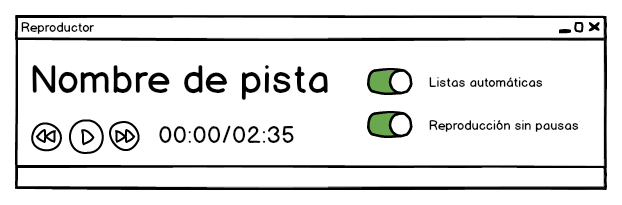
\includegraphics[width=15cm]{./Figuras/window}
\caption[Interfaz de usuario]{La interfaz de usuario utiliza controles simples para evitar complicaciones de uso.}
\label{fig:inter}
\end{figure}

\noindent El software tiene una interfaz simple, consta de un bot\'on de reproducci\'on/pausa y un par de botones para la pista siguiente y la anterior. Muestra una etiqueta para el nombre del archivo en reproducci\'on y una para el tiempo restante. Tambi\'en se tiene un par de botones para activar la generaci\'on de listas de reproducci\'on autom\'atica y la reproducci\'on sin pausa.

%\porHacer{M\'as elementos de interfaz se podr\'ian agregar en el futuro.} 

\subsection{Funcionamiento interno}

Las funciones principales del software son tres:

\begin{description}
\item[Reproducci\'on de archivos.]{La funci\'on b\'asica es la de reproducir archivos en formato {\sc WAV} sin compresi\'on.}
\item[Generaci\'on de listas de reproducci\'on.]{Un generador de listas basado en la inforaci\'on obtenida del procesamiento de cada archivo. Mediante un algoritmo de b\'usqueda de similitudes entre los datos se puede encontrar la siguiente pista a reproducir.}
\item[Transici\'on inteligente.]{Al estar activa la opci\'on de reproducci\'on sin pausa, las pistas tendr\'an una trnasici\'on suave entre inicio y fin. La selecci\'on de los puntos de transici\'on se hace mediante un algoritmo que reconoce un punto entre dos pistas que tiene un ritmo que sea semejante.}
\end{description}

\noindent En la figura \ref{fig:func} se muestra un diagrama del funcionamiento del software.

\begin{figure}[h!]
\centering
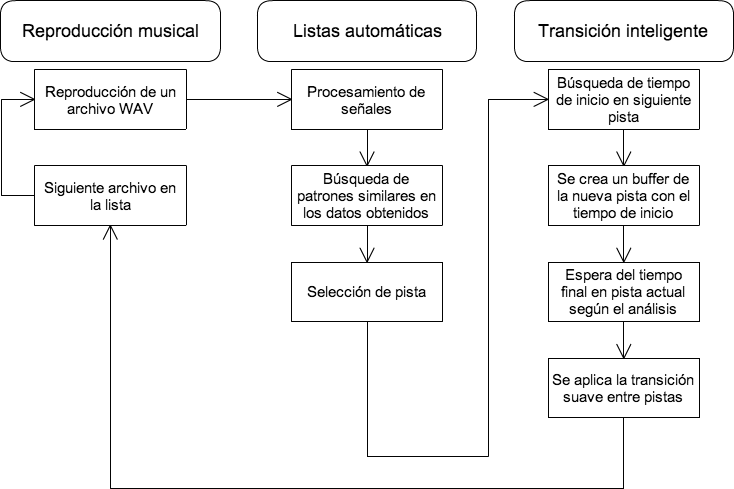
\includegraphics[width=15cm]{./Figuras/diagram1}
\caption[Funcionamiento del software]{Funciones principales del software.}
\label{fig:func}
\end{figure}

\section{Obtenci\'on de informaci\'on relevante}

Para poder generar una lista de reproducci\'on basada en el ritmo de las pistas es necesario procesar \'estas antes. Para ello es necesario utilizar la transformada r\'apida de Fourier con la cual se obtiene informaci\'on de las frecuencias individuales en un tiempo $t$. El proceso de obtenci\'on de informaci\'on relevante consiste en capturar en ventanas de tiempo constantes la informaci\'on de las frecuencias, al t\'ermino de cada ventana de tiempo se hace una selecci\'on l\'ogica por medio de votaciones. Los valores en tiempo $t_1$ mayores a los del tiempo $t_0$ dan un voto positivo, los menores dan un voto negativo, al final se cuentan los votos de la ventana de tiempo y si la mayor\'ia son positivos entonces se almacena el valor actual, de no serlo simplemente se continua a la pr\'oxida ventana de tiempo.

\noindent La l\'ogica anterior se basa en que la pista presenta intensidades propias de su ritmo, la intenci\'on es capturar los momentos en que ocurre un cambio de intensidades para comparar con otras pistas y encontrar aquellas que sean compatibles en ritmo.

\noindent Ya que al reproducir una pista es necesario obtener de ella sus datos en formato PCM, \'estos se utilizan para realizar el proceso de obtenci\'on de informaci\'on en forma paralela a la reproducci\'on, cada instante de tiempo se actualizan estos datos, de esa manera se asegura que el tiempo de obtenci\'on sea equivalente al de la pista. Los datos obtenidos se almacenan en un archivo de texto plano.

\begin{landscape}
\begin{figure}
\centering
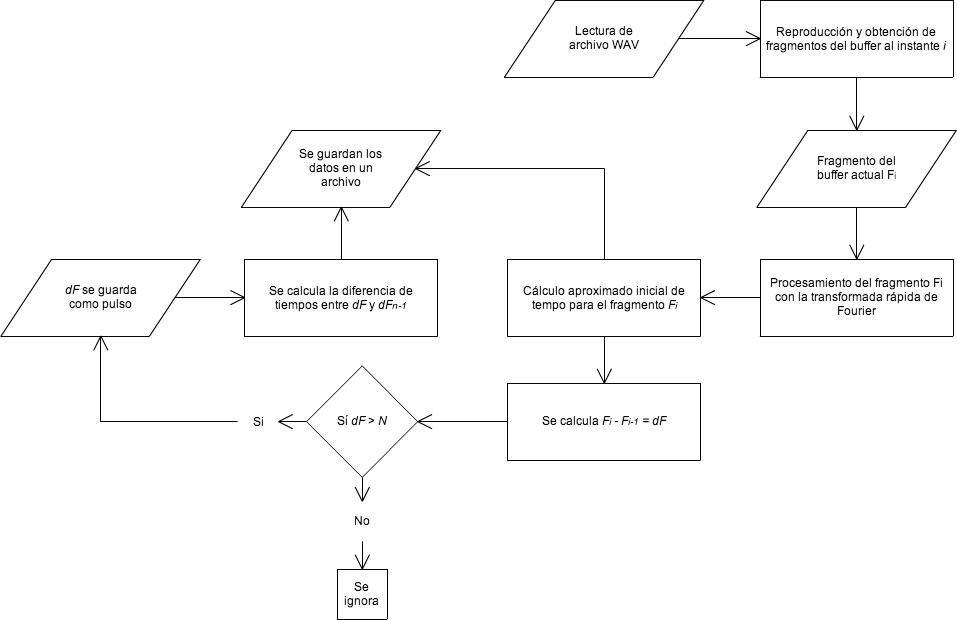
\includegraphics[width=22cm]{./Figuras/diagram2}
\caption[Obtenci\'on de informaci\'on]{Obtenci\'on de informaci\'on relevante de la pista.}
\label{fig:diaginfo}
\end{figure}
\end{landscape}

\section{Generaci\'on de listas de reproducci\'on}

La selecci\'on de pistas se realiza mediante un an\'alisis de datos que corre en paralelo con la reproducci\'on actual. Cada pista que se reproduce tiene un archivo de informaci\'on obtenida y se utiliza para comparar la pista correspondiente con las pistas en el directorio. La rutina que compara los datos entre pistas consiste en buscar un patr\'on de comportamiento en los datos, primero se buscan patrones en el archivo de datos de la pista en reproducci\'on, es decir, buscar secciones en los datos que sean coincidentes, se almacena el patr\'on y se guardan los tiempos en que ocurre el patr\'on encontrado. Con esa informaci\'on se procede a analizar los archivos de datos de las pistas en el directorio, por cada an\'alisis se realiza una rutina de comparaci\'on entre los datos de la pista actual $p_r$ y los de la candidata $p_c$. El an\'alisis consiste en comparar los datos de ambas pistas de tal manera que sigan un patr\'on de subidas y bajadas en los valores de los datos; si el valor de $p_{ri}$ y el valor de $p_{ci}$ son al mismo tiempo mayores o menores que $p_{ri-1}$ y $p_{ci-1}$ respectivamente entonces los patrones son compatibles y se procede a comparar los siguientes valores, en caso de que $p_{ri-1}$ sea mayor que su valor anterior y $p_{ci-1}$ menor al suyo entonces el patr\'on ya no es aceptable si se procede a analizar a otro patr\'on.

\noindent Con esa informaci\'on se obtienen los tiempos donde hay patrones compatibles entre la pista actual y la candidata, ahora solo queda seleccionar el que mejor se adapte. Normalmente cada pista tiene varios patrones candidatos, el mejor de ellos debe tener un equilibrio entre posici\'on temporal en ambas pistas y de precisi\'on entre patrones de la pista actual y la candidata. La pista seleccionada debe de cumplir los mismos criterios, pero esta vez entre los patrones seleccionados de cada pista anteriormente.

\noindent La primera vez que se utiliza una pista no es posible obtener su informaci\'on hasta que se haya terminado de reproducir, por lo que se utiliza la informaci\'on obtenida hasta el momento para seleccionar una pista compatible en ritmo sin pasar por todos los filtros.

\noindent Si por alguna raz\'on no se encuentra una pista ya sea por que no es compatible o por alg\'un error interno, entonces se selecciona una pista al azar.

\noindent La lista de reproducci\'on se va generando conforme avanza la reproducci\'on, para evitar repeticiones, se tiene una {\em lista tab\'u}\footnote{Una {\em lista tab\'u} es una lista que se guarda en memoria durante un proceso para almacenar datos del m\'ismo con la intenci\'on de evitar repetirlos.} que se actualiza con las pistas previas hasta que se tenga una lista con todas las pistas del directorio actual.
\begin{landscape}
\begin{figure}
\centering
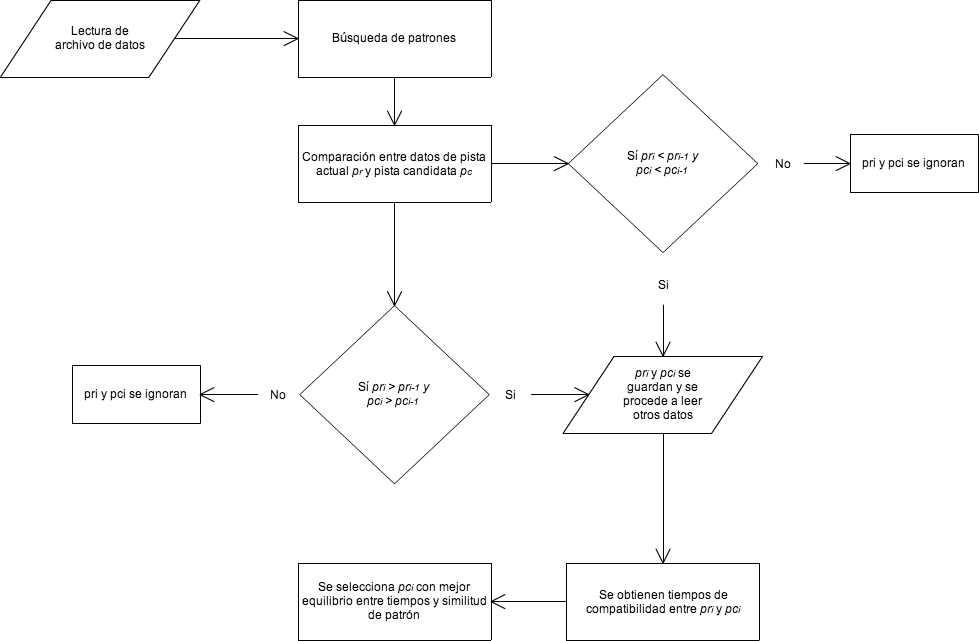
\includegraphics[width=22cm]{./Figuras/diagram3}
\caption[Generaci\'on de listas de reproducci\'on]{Diagrama que muestra la forma en que se generan las listas.}
\label{fig:diaglist}
\end{figure}
\end{landscape}
\section{Transici\'on inteligente entre pistas}

Una de los datos obtenidos del an\'alisis de la pista seleccionada es el tiempo en que ocurre el patr\'on encontrado, tanto en la pista actual como en la seleccionada, este dato describe el instante en la pista actual en que se puede iniciar una transici\'on de salida para la pista actual combinado con una de entrada para la nueva pista, de la cual tambi\'en se conoce el tiempo en que ocurrir\'ia la transici\'on.

\section{Dificultades}

Durante el desarrollo del proyecto presentaron varias dificultades; la b\'usqueda un m\'etodo eficiente para obtener datos de procesamiento, el intercambio de informaci\'on entre hilos sin afectar el flujo principal, efectuar transiciones sin perder informaci\'on de procesamiento entre pistas, entre otros problemas menores.

\noindent El principal problema fue el manejo de hilos en el programa; al realizar distintas actividades en el sistema operativo se generaban peque\~nas p\'erdidas de datos y pausas en la reproducci\'on que afectaban al an\'alisis. La soluci\'on fue utilizar subprocesos que corren de forma independiente del programa en segundo plano para evitar interferencias. Los subprocesos son programas independientes por lo tanto se pueden escribir en cualquier lenguaje distinto a la implementaci\'on principal, lo que aumenta la eficiencia en general.
\chapter{Evaluaci\'on}
\label{chap:eval}
%\porHacer{La evaluaci\'on est\'a en proceso. Algunos experimentos podr\'ian cambiar. (2 semanas desde hoy aprox.)}

Para un completo desarrollo de software es necesario realizar pruebas de software, con los cuales es posible detectar errores, defectos o vulnerabilidades que se pueden reparar para ofrecer un mejor funcionamiento. En este caso se realizan dos tipos de pruebas; las pruebas de rendimiento, que consisten en pruebas que se ejecutan por si solas y que arrojan un resultado cuantificable y pruebas con usuarios, en las cuales se les pide a los usuarios realizar ciertas acciones con el programa y evaluar tales acciones.

\section{Dise\~no experimental}
Para el funcionamiento adecuado del software se utilizaron varios m\'etodos que logran un flujo ininterrumpido pero que requieren m\'as recursos. Para evaluar el rendimiento del software bajo \'estas circunstancias, se toman en cuenta los siguientes criterios: 
\begin{description}
\item [Velocidad de procesamiento]{Se eval\'ua la velocidad que el software necesita para realizar las operaciones necesarias. Dependiendo de la plataforma y el hardware en que se ejecuta el software podr\'ian existir diferencias de velocidad.}
\item [Precisi\'on algor\'itmica]{El software genera datos en base a informaci\'on obtenida del procesamiento. La modificaci\'on de uno o varios par\'ametros en los algoritmos genera datos distintos. En este caso se eval\'uan las condiciones en las que opera el software y que tan precisos son los datos generados.}
\item [Eficiencia de ejecuci\'on]{El procesamiento, an\'alisis y reproducci\'on trabajan en tiempo real, representan una carga de memoria. Para este criterio se eval\'ua la eficiencia en que trabaja el software en distintas condiciones de plataforma y hardware, as\'i como el uso de hilos.}
\end{description}

\noindent Estas pruebas se realizan mediante rutinas que ejecutan m\'etodos espec\'ificos del software o ejecuci\'on completa, siempre con par\'ametros cambiantes. Se llevan a cabo en plataformas distintas bajo circunstancias de hardware variadas (ejecuci\'on \'unica, ejecuci\'on junto a otros programas, etc\'etera).

\noindent Adicionalmente a las pruebas de rendimiento se realizan pruebas b\'asicas con usuarios donde se eval\'uan los siguientes criterios:

\begin{description}
\item [Generaci\'on autom\'atica de listas de reproducci\'on]{De forma similar a la precisi\'on algor\'itmica, pero desde el punto de vista de los usuarios. La intenci\'on es evaluar el grado en que se seleccionan las pistas y la fidelidad del ritmo musical.}
\item [Transici\'on y mezclado entre pistas]{En este criterio se eval\'ua el grado de aceptaci\'on por parte de los usuarios de la funci\'on de mezclado inteligente utilizando efectos de transici\'on entre pistas.}
%\item [Interfaz gr\'afica]{Aunque no es la intenci\'on principal de la tesis, tambi\'en se eval\'uan aspectos de usabilidad. El objetivo de este criterio es analizar tendencias por parte de los usuarios para un futuro proyecto.}
\end{description}

\subsection{Velocidad de procesamiento}

Esta prueba consiste en experimentar con el tiempo que le toma al software procesar los archivos para una sola pista. Se realizara de dos modos: sin reproducci\'on y con reproducci\'on. Cuando se realiza sin reproducci\'on, el software no tomar\'a en cuenta la pista sino que pasar\'a directo al procesamiento de datos y se ejecutar\'a hasta acabar por completo con todos los archivos. Cuando se realiza con reproducci\'on, el software utiliza un limite de archivos para asegurar terminar antes de que la pista actual finalice.

\noindent Para cada uno de los modos se hacen de 20 a 30 repeticiones y en el caso de el modo sin reproducci\'on se utilizan de 50 a 100 archivos de prueba.

\subsection{Precisi\'on algor\'itmica}

Muchos de los elementos dentro del algoritmo son constantes que se han elegido en base al comportamiento buscado, sin embargo, muchas de estas constantes parecen ser m\'as favorables en ciertas ocasciones. En esta prueba se experimenta con la precisi\'on de los algoritmos cuando sus constantes son cambiadas, para medir la precisi\'on se utiliza una lista de reproducci\'on modelo, la cual consiste en pistas que van cambiando sus bpm de forma progresiva. Se realizan de 20 a 30 repeticiones por cada cambio.

\subsection{Eficiencia de ejecuci\'on}

Con las pruebas anteriores ahora se tiene la mejor configuraci\'on de funcionamiento para el software, ahora se experimenta con \'esta la eficiencia de ejecuci\'on donde se eval\'ua la cantidad de recursos m\'inima y m\'axima que necesita el software para funcionar. De igual manera se realizan de 20 a 30 repeticiones con y sin reproducci\'on y para el modo sin reproducci\'on se utilizan de 50 a 100 archivos de prueba.

\subsection{Generaci\'on autom\'atica de listas de reproducci\'on}

Las pruebas con usuarios son m\'as enfocadas al uso del software y no al funcionamiento interno. En el caso de la prueba de generaci\'on de listas de reproducci\'on el usuario eval\'ua desde su punto de vista que eficiente es el software en cuanto a selecci\'on de pistas. Se utilizan pistas seleccionadas por el propio usuario y al final se le har\'a una encuesta pregunt\'andole sobre la eficiencia de la generaci\'on autom\'atica de listas de reproducci\'on.

\subsection{Transici\'on y mezclado entre pistas}

Durante la prueba se le pide al usuario que active la funci\'on de transici\'on y mezclado y que escuche fragmentos de pistas. El usuario eval\'ua esta funci\'on dando a conocer que tan eficiente es y si es de su agrado.

%\subsection{Interfaz gr\'afica}

%\porHacer{El usuario eval\'ua la facilidad con la que se utiliza el programa. Se abre un espacio para cr\'iticas y sugerencias. (Hay posibilidades de que esta prueba no se realice pues el enfoque actual no incluye una interfaz gr\'afica intuitiva.)}

\section{Resultados}

Despu\'es de realizar las pruebas, se eval\'uan los resultados obtenidos. En el caso de las pruebas de rendimiento, se generaron {\em scripts}\footnote{Un {\em script} es un conjunto de instrucciones interpretadas por el sistema operativo para realizar tareas simples.} que corren solo ciertas partes del programa y guardan informaci\'on. Las pruebas con usuarios fueron independeintes, a cada usuario se le dieron tareas a realizar con el programa y evaluarlas al t\'ermino de cada una.

\subsection{Pruebas de rendimiento}

En total se realizaron tres pruebas de rendimiento. Cada prueba se realiza en las plataformas {\sc Linux}\footnote{{\sc Linux} es un sistema operativo de libre distribuci\'on basado en {\sc Unix} (otro sistema operativo de libre distribuci\'on), desarrollado originalmente por Linus Torvalds.}, {\sc Windows}\footnote{{\sc Microsoft Windows} es el nombre de una familia de sistemas operativos desarrollados y vendidos por {\sc Microsoft}.} y {\sc OS X}\footnote{{\sc OS X}, antes llamado {\sc Mac OS X}, es una serie de sistemas operativos basados en {\sc Unix} desarrollados, comercializados y vendidos por {\sc Apple Inc.} que ha sido incluido en su gama de computadoras {\sc Macintosh} desde el a\~no de 2002.} (excepto la prueba de presici\'on algor\'itmica), en cada plataforma se realiza la prueba sin procesos en ejecuci\'on (correr el programa con la mayor cantidad de memoria disponible) y con varios procesos en ejecuci\'on (correr el programa solo con memoria suficiente). La cantidad de repeticiones depende de cada prueba, rondando entre las 50 y 100 repeticiones.

\noindent La prueba de velocidad de procesamiento se efect\'ua tomando los tiempos que tarda el programa para generar los datos, procesarlos, compararlos y dar una respuesta; en este caso la respuesta es la siguiente pista a reproducir.

\noindent En el caso de la prueba de precisi\'on algor\'itmica se modifican aspectos internos; como un umbral de reconocimiento utilizado para suavizar los valores y hacer m\'as facil el reconocimiento, o el n\'umero de bandas de frecuencia que afectan la precisi\'on con la que se procesa la informaci\'on. El porcentaje de aserci\'on se eval\'ua con una lista de reproducci\'on predeterminada; entre m\'as fiel sea la lista de reproducci\'on generada a la predeterminada, mayor ser\'a su porcentaje de aserci\'on.

\noindent Utilizando la mejor configuraci\'on de la prueba de precisi\'on algor\'itmica, se efect\'ua una prueba de eficiencia de ejecuci\'on, simplemente se ejecuta el programa bajo distintas circunstancias y se toman los datos directamente del sistema operativo.

\subsection{Pruebas con usuarios}
Para las pruebas con usuarios se realizar\'a una sola ejecuci\'on por usuario y al final se le pedir\'a llenar una encuesta. La cantidad m\'inima de usuarios ser\'a 20 (10 mujeres y 10 hombres, 10 j\'ovenes y 10 adultos).

\noindent Para la prueba de generaci\'on autom\'atica de listas de reproducci\'on, se di\'o a los usuarios la tarea de escuchar una de las pistas disponibles y evaluar el nivel en que el programa selecciona autom\'aticamente las pistas.

\noindent Despu\'es de la evaluaci\'on anterior, los usuarios evaluaron los efectos de transici\'on y mezclado entre las pistas.

\porHacer{Los datos reales a\'un no se tienen, se pretende tenerlos listos entre finales de Junio y mitad de Julio, tiempo en el que se pretende tener las pruebas completas y tener las suficientes encuestas. A continuaci\'on se presentan los cuadros y figuras donde estar\'an los resultados reales pero con valores provisionales que no reflejan nada.}

%\noindent Finalmente se les di\'o la tarea de evaluar la facilidad con la que utilizaron el programa.

%\porHacer{Probablemente se agreguen m\'as pruebas o se modifiquen algunas existentes.}

\newpage

\renewcommand\arraystretch{1.3}
\begin{table}[t]
	\centering
  	\caption[Velocidad de procesamiento]{Comparativa de velocidad de procesamiento usando distintos parametros tanto de hardware como de software. \porHacer{(Datos provisionales)}}
  	\scalebox{0.8}{
  	\begin{tabular}{| p{4cm} | p{4cm} | p{4cm} |}
  			\hline
  			\footnotesize \begin{minipage}[c][40pt][c]{20pt} \textbf{Sistema \mbox{operativo}}\end{minipage} &
			\footnotesize \begin{minipage}[c][40pt][c]{20pt} \textbf{\mbox{Tiempo de} \mbox{procesamiento} \mbox{sin reproducci\'on}}\end{minipage} &
			\footnotesize \begin{minipage}[c][40pt][c]{20pt} \textbf{\mbox{Tiempo de} \mbox{procesamiento} \mbox{con reproducci\'on}}\end{minipage}\\
  			\hline
			\multicolumn{3}{|l|}{
  				\begin{minipage}{15cm}
    					Junto a varios procesos
  				\end{minipage}
			}\\
  			\hline
  			Mac OS X & 
			\mbox{\porHacer{0.0 s}} & 
			\mbox{\porHacer{0.0 s}}\\
  			Ubuntu & 
			\mbox{\porHacer{0.0 s}} & 
			\mbox{\porHacer{0.0 s}}\\
  			Windows & 
			\mbox{\porHacer{0.0 s}} & 
			\mbox{\porHacer{0.0 s}}\\
			\hline
			\multicolumn{3}{|l|}{
  				\begin{minipage}{15cm}
    					Proceso \'unico
  				\end{minipage}
			}\\
			\hline
			Mac OS X & 
			\mbox{\porHacer{0.0 s}} & 
			\mbox{\porHacer{0.0 s}}\\
  			Ubuntu & 
			\mbox{\porHacer{0.0 s}} & 
			\mbox{\porHacer{0.0 s}}\\
  			Windows & 
			\mbox{\porHacer{0.0 s}} & 
			\mbox{\porHacer{0.0 s}}\\
			\hline
 		\end{tabular}
  		}
	\label{table:eva-vel}
\end{table}
\begin{table}[t]
	\centering
  	\caption[Precisi\'on algor\'itmica]{Se compara la precisi\'on con la que el programa acierta en la selecci\'on autom\'atica de pistas. \porHacer{(Datos provisionales)}}
  	\scalebox{0.8}{
  	\begin{tabular}{| p{4cm} | p{4cm} | p{4cm} | p{4cm} |}
  			\hline
  			\footnotesize \begin{minipage}[c][40pt][c]{20pt} \textbf{Umbral de \mbox{reconocimiento}}\end{minipage} &
			 \footnotesize \begin{minipage}[c][40pt][c]{20pt} \textbf{\mbox{N\'umero de} \mbox{bandas de} \mbox{frecuencia}}\end{minipage} &
			\footnotesize \begin{minipage}[c][40pt][c]{20pt} \textbf{\mbox{Porcentaje de} \mbox{aserci\'on} \mbox{sin reproducci\'on}}\end{minipage} &
			\footnotesize \begin{minipage}[c][40pt][c]{20pt} \textbf{\mbox{Porcentaje de} \mbox{aserci\'on} \mbox{con reproducci\'on}}\end{minipage}\\
  			\hline
			& 4 & 
			\mbox{\porHacer{0.0}} & 
			\mbox{\porHacer{0.0}}\\
  			Sin umbral & 8 & 
			\mbox{\porHacer{0.0}} & 
			\mbox{\porHacer{0.0}}\\
  			& 16& 
			\mbox{\porHacer{0.0}} & 
			\mbox{\porHacer{0.0}}\\
			\hline
  			& 4 & 
			\mbox{\porHacer{0.0}} & 
			\mbox{\porHacer{0.0}}\\
  			5 unidades & 8 & 
			\mbox{\porHacer{0.0}} & 
			\mbox{\porHacer{0.0}}\\
  			& 16& 
			\mbox{\porHacer{0.0}} & 
			\mbox{\porHacer{0.0}}\\
			\hline
  			& 4 & 
			\mbox{\porHacer{0.0}} & 
			\mbox{\porHacer{0.0}}\\
  			10 unidades & 8 & 
			\mbox{\porHacer{0.0}} & 
			\mbox{\porHacer{0.0}}\\
  			& 16& 
			\mbox{\porHacer{0.0}} & 
			\mbox{\porHacer{0.0}}\\
			\hline
 		\end{tabular}
  		}
	\label{table:eva-alg}
\end{table}
\begin{table}[t]
	\centering
  	\caption[Eficiencia de ejecuci\'on]{Se comparan los resultados obtenidos y se analizan los recursos utilizados en cada sistema operativo. \porHacer{(Datos provisionales)}}
  	\scalebox{0.8}{
  	\begin{tabular}{| p{4cm} | p{5cm} | p{4cm} |}
  			\hline
  			\footnotesize \begin{minipage}[c][40pt][c]{20pt} \textbf{Sistema \mbox{operativo}}\end{minipage} &
			\footnotesize \begin{minipage}[c][40pt][c]{20pt} \textbf{\mbox{Recursos utilizados} \mbox{por el sistema operativo} \mbox{sin reproducci\'on}}\end{minipage} &
			\footnotesize \begin{minipage}[c][40pt][c]{20pt} \textbf{\mbox{Recursos utilizados} \mbox{por el sistema operativo} \mbox{con reproducci\'on}}\end{minipage}\\
  			\hline
			\multicolumn{3}{|l|}{
  				\begin{minipage}{15cm}
    					Junto a varios procesos
  				\end{minipage}
			}\\
  			\hline
  			Mac OS X & 
			\mbox{\porHacer{0.0}} & 
			\mbox{\porHacer{0.0}}\\
  			Ubuntu & 
			\mbox{\porHacer{0.0}} & 
			\mbox{\porHacer{0.0}}\\
  			Windows & 
			\mbox{\porHacer{0.0}} & 
			\mbox{\porHacer{0.0}}\\
			\hline
			\multicolumn{3}{|l|}{
  				\begin{minipage}{15cm}
    					Proceso \'unico
  				\end{minipage}
			}\\
			\hline
			Mac OS X & 
			\mbox{\porHacer{0.0}} & 
			\mbox{\porHacer{0.0}}\\
  			Ubuntu & 
			\mbox{\porHacer{0.0}} & 
			\mbox{\porHacer{0.0}}\\
  			Windows & 
			\mbox{\porHacer{0.0}} & 
			\mbox{\porHacer{0.0}}\\
			\hline
 		\end{tabular}
  		}
	\label{table:eva-eje}
\end{table}

\newpage

\begin{figure}[t]
\begin{center}
\scalebox{1.6}{
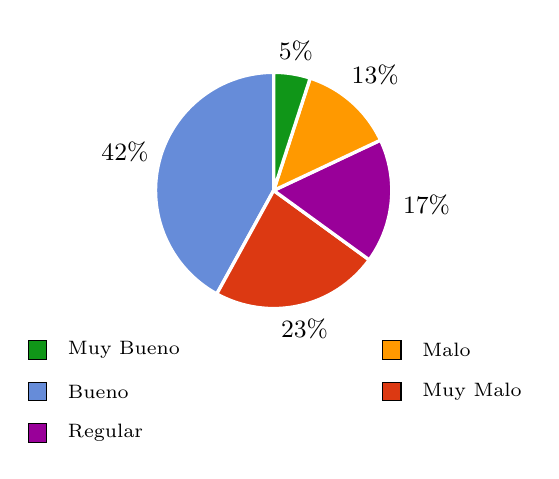
\begin{tikzpicture}
[
    pie chart,
    slice type={comet}{blu},
    slice type={legno}{rosso},
    slice type={coltello}{giallo},
    slice type={sedia}{viola},
    slice type={caffe}{verde},
    pie values/.style={font={\small}},
    scale=1.5
]

    \pie[xshift=2.0cm,
    	values of coltello/.style={pos=1.3}, 
    	values of legno/.style={pos=1.2},
   	values of comet/.style={pos=1.3},
   	values of sedia/.style={pos=1.3},
   	values of caffe/.style={pos=1.2} ]%
        { }{42/comet,23/legno,17/sedia,13/coltello,5/caffe}

    \legend[shift={(0cm,-1cm)}]{{Muy Bueno}/caffe, {Bueno}/comet, {Regular}/sedia}
    \legend[shift={(3cm,-1cm)}]{{Malo}/coltello, {Muy Malo}/legno}

\end{tikzpicture}
}
\end{center}
\caption[Fidelidad de generaci\'on de listas de reproducci\'on]{Nivel de fidelidad de generaci\'on autom\'atica de listas seg\'un los usuarios. \porHacer{(Datos provisionales)}}
\label{fig:us-fid}
\end{figure}
\begin{figure}[t]
\begin{center}
\scalebox{1.6}{
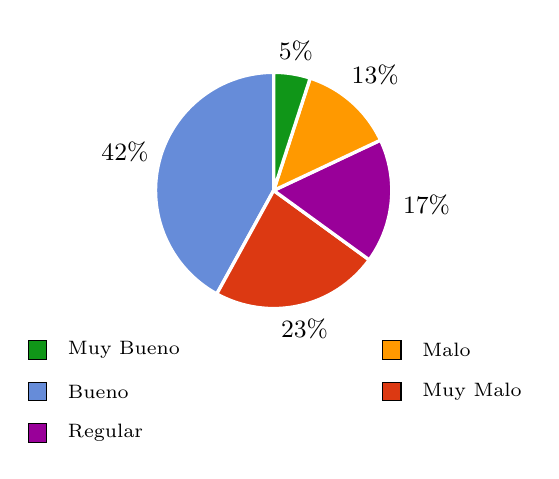
\begin{tikzpicture}
[
    pie chart,
    slice type={comet}{blu},
    slice type={legno}{rosso},
    slice type={coltello}{giallo},
    slice type={sedia}{viola},
    slice type={caffe}{verde},
    pie values/.style={font={\small}},
    scale=1.5
]

    \pie[xshift=2.0cm,
    	values of coltello/.style={pos=1.3}, 
    	values of legno/.style={pos=1.2},
   	values of comet/.style={pos=1.3},
   	values of sedia/.style={pos=1.3},
   	values of caffe/.style={pos=1.2} ]%
        { }{42/comet,23/legno,17/sedia,13/coltello,5/caffe}

    \legend[shift={(0cm,-1cm)}]{{Muy Bueno}/caffe, {Bueno}/comet, {Regular}/sedia}
    \legend[shift={(3cm,-1cm)}]{{Malo}/coltello, {Muy Malo}/legno}

\end{tikzpicture}
}
\end{center}
\caption[Efecto de transici\'on y mezclado]{Nivel de ejecuci\'on de efectos de transici\'on y mezclado seg\'un los usuarios. \porHacer{(Datos provisionales)}}
\label{fig:us-tm}
\end{figure}
%\begin{figure}[t]
\begin{center}
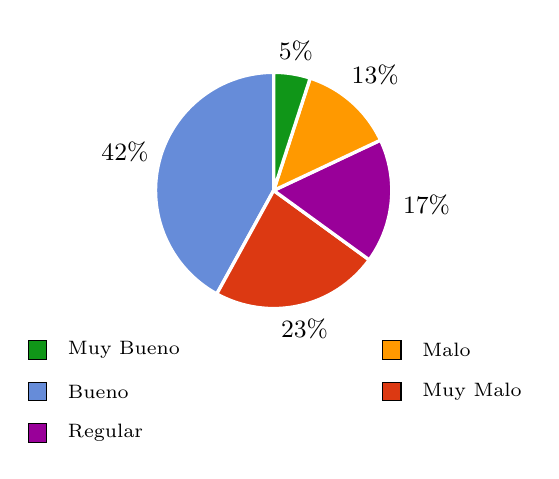
\begin{tikzpicture}
[
    pie chart,
    slice type={comet}{blu},
    slice type={legno}{rosso},
    slice type={coltello}{giallo},
    slice type={sedia}{viola},
    slice type={caffe}{verde},
    pie values/.style={font={\small}},
    scale=1.5
]

    \pie[xshift=2.0cm,
    	values of coltello/.style={pos=1.3}, 
    	values of legno/.style={pos=1.2},
   	values of comet/.style={pos=1.3},
   	values of sedia/.style={pos=1.3},
   	values of caffe/.style={pos=1.2} ]%
        { }{42/comet,23/legno,17/sedia,13/coltello,5/caffe}

    \legend[shift={(0cm,-1cm)}]{{Muy Bueno}/caffe, {Bueno}/comet, {Regular}/sedia}
    \legend[shift={(3cm,-1cm)}]{{Malo}/coltello, {Muy Malo}/legno}

\end{tikzpicture}
\end{center}
\caption[Facilidad de uso del programa]{Nivel usabilidad seg\'un los usuarios. \porHacer{(Datos provisionales)}}
\label{fig:us-gui}
\end{figure}

\section{An\'alisis de resultados}

Con el an\'alisis de resultados se obtienen respuestas que describen el funcionamiento del software en situaciones distintas. La modificaci\'on de ciertas variables genera un flujo de ejecuci\'on muy distinto, algunas veces favorable para la misma.

\noindent A continuaci\'on se muestra el an\'alisis de cada prueba, los factores cambiantes en cada una y el objetivo de su realizaci\'on.

\subsection{An\'alisis de rendimiento}

El cuadro \ref{table:eva-vel} muestra los resultados de la prueba de velocidad de procesamiento, \'esta fue realizada para conocer el tiempo que necesita el software para dar una respuesta. Las pistas de audio tienen longitudes variables y gran parte de las operaciones del software dependen de \'esta; el an\'alisis principal consiste en dividir la pista en bloques de tama\~no constante y el n\'umero de bloques depende de la longitud de la pista, la detecci\'on de patrones consiste en analizar archivos generados por la operaci\'on anterior  y su tama\~no es proporcional a la longitud de la pista. Si una pista es de gran longitud entonces tardar\'a m\'as en realizar el procesamiento, por ello es necesario realizar todas las tareas involucradas en un hilo distinto al principal. La intenci\'on de esta prueba es asegurar que el hilo de procesamiento termina antes que la reproducci\'on para tener una respuesta a la siguiente pista.

\noindent Las pruebas iniciales muestran que la velocidad de procesamiento es afectada por la reproducci\'on de la pista, es por eso que se eval\'ua la velocidad que toma el procesamiento con y sin reproducci\'on de pista. \'esto es debido a que la reproducci\'on tambi\'en ocurre en un hilo distinto al principal y toma parte de los recursos para ejecutarse.

\noindent En el cuadro \ref{table:eva-alg} se muestran los resultados de la prueba de precisi\'on algor\'itmica que consiste en analizar las respuestas obtenidas del software bajo ciertas condiciones cambiantes con la intenci\'on de que los datos permanezcan sin cambios. En caso de que existan cambios se toma como mejor condici\'on aquella que tenga cambios m\'inimos.

\noindent Para esta prueba se tiene una lista de reproducci\'on est\'atica como modelo que contiene pistas en una sucesi\'on que sigue una l\'ogica, tal sucesi\'on consiste en pistas de prueba que incrementan sus bpm conforme avanza en la lista. Uno de los factores para esta prueba es el umbral de reconocimiento, \'este es un valor constante que suaviza los valores obtenidos del procesamiento para tener un mejor rango de reconocimiento de bpm, modificar este valor puede conllevar a cambios en la forma en que se genera el archivo de an\'alisis y por lo tanto en la forma de detectar patrones en las pistas. Otro factor a tomar en cuenta es la cantidad de bandas utilizadas, entre mayor sea la cantidad menos sensible es el software pero m\'as r\'apida es su ejecuci\'on, para la prueba de velocidad se utilizaron 8 bandas, para esta prueba se utilizan 4, 8 y 16 bandas. Por \'ultimo se ejecuta la prueba con y sin reproducci\'on para analizar si \'esto afecta la forma en que se genera una respuesta.

\noindent En el cuadro \ref{table:eva-eje} se muestra la evaluaci\'on de la prueba de eficiencia de ejecuci\'on, \'esta sirve para conocer la cantidad de recursos que utiliza el software al ejecutarse en distintos entornos y bajo condiciones de mucha o poca memoria. La intenci\'on es llevar al l\'imite al software y saber hasta que punto a\'un puede continuar operando de forma constante como en las pruebas anteriores. Es importante saber cual es el requerimiento m\'inimo y m\'aximo del software para asegurar el mejor funcionamiento posible y no interferir el la ejecuci\'on de otros procesos.

\subsection{An\'alisis con usuarios}

En los resultados de la prueba de generaci\'on autom\'atica de listas de reproducci\'on mostrados en la figura \ref{fig:us-fid}, los usuarios tienen la tarea de evaluar el seguimiento r\'itmico de la lista de reproducci\'on. 

\noindent Para la prueba se utiliza una lista pregenerada con pistas de prueba y una lista de reproducci\'on que se generar\'a en el momento. Al final de la prueba se le pedir\'a al usuario calificar la fidelidad musical; es decir, si el software logr\'o generar una lista de acuerdo a los ritmos.

\noindent Esta prueba es muy variable en sus resultados y depende de los gustos de cada usuario, pero es importante conocer estos datos para saber si el software realmente cumple con su funci\'on.

\noindent En la figura \ref{fig:us-tm} se muestran los resultados de la prueba de transici\'on y mezclado entre pistas, \'esta pone a los usuarios en la tarea de evaluar la funci\'on del software para generar una transici\'on entre dos pistas. Para ello se reproduce una lista pregenerada y una generada en el momento. Los usuarios eval\'uan si la funci\'on se ejecuta de forma adecuada.

%\noindent Finalmente se muestra la figura \ref{fig:us-gui} de la prueba de usabilidad, \'esta consiste en evaluar la facilidad de uso del software durante la realizaci\'on de las tareas. El objetivo principal del proyecto no se enfoca en la interfaz gr\'afica, sin embargo como trabajo a futuro es importante tomar este aspecto en cuenta.

%\noindent Adicionalmente a las pruebas se le pide a los usuarios que mencionen aspectos destacables tanto positivos como negativos del software y que les gustar\'ia ver en \'el.
\chapter{Conclusiones}
\label{chap:conc}
\porHacer{Este cap\'itulo necesita datos de la evaluaci\'on, por lo tanto est� sujeto a cambios dependiendo de los resultados. Se marca en rojo lo que tenga m\'as probabilidad de ser cambiado.}

Durante el desarrollo de este proyecto se present\'o un software con la capacidad de analizar pistas de audio para obtener informaci\'on del ritmo y de esa manera generar listas de reproducci\'on basadas en tal caracter\'istica. La finalidad de la herramienta es brindar una mejor experiencia de reproducci\'on musical para el usuario.

\noindent Se implementaron m\'etodos de an\'alisis de se\~nales y detecci\'on de patrones, los cuales permiten detectar la velocidad del ritmo e inicio y final de pista con los que se generan listas de reproducci\'on de forma autom\'atica.

\noindent Para producir una mejor experiencia de reproducci\'on musical se implementaron efectos de transici\'on entre pistas; entre dos pistas se calcula un momento temporal en el que los ritmos son similares, se aplica un efecto de difuminaci\'on en la primera pista que disminuye su potencia, mientras la segunda pista la aumenta con un efecto similar.

\noindent El desarrollo principal se realiz\'o en el lenguaje de programaci\'on {\sc Python} mientras que algunas rutinas de procesamiento se realizaron en el lenguaje de programaci\'on {\sc Java} debido a la carga algor\'itmica.

\section{Discusi\'on}

El prototipo de software desarrollado demuestra que sus resultados son favorables en cuanto a su objetivo, de acuerdo con los usuarios que lo probaron. La generaci\'on de listas respeta el ritmo de las pistas y se crea una lista con una suceci\'on l\'ogica de pistas.

%\porHacer{(ALT) El prototipo de software desarrollado demuestra que sus resultados son inexactos ya que no cumplen con el objetivo, de acuerdo con los usuarios que lo probaron. La generaci\'on de listas es inexacta y no respeta el ritmo en la mayor\'ia de las veces.}

\noindent \porHacer{Aunque las transiciones entre pistas son efectos que intentan mejorar la experiencia del usuario, no a todos les convence esta caracter\'istica, algunos usuarios prefirieron desactivar la caracter\'istica, a otros usuarios les agrad\'o la idea pero piensan que se puede mejorar la detecci\'on del tiempo correcto en que se debe realizar.}% (Es probable que no a todos les guste esta caracter\'istica, se definir\'a despues de semana santa)}

\noindent De acuerdo con los usuarios, la interfaz no est\'a muy elaborada, pero es sencilla de utilizar pues sus controles se reconocen a simple vista y sus opciones se pueden identificar unas de otras facilmente.

\noindent Aunque los resultados de ejecuci\'on del software son los esperados, existen problemas de velocidad de procesamiento que causan conflictos entre los hilos del software; el procesamiento en tiempo real se vuelve muy pesado en funci\'on al n\'umero de archivos de sonido en un directorio. Debido a que la restricci\'on de tiempo se define por la duraci\'on de la pista actual, un alternativa viable a la ejecuci\'on en tiempo real de este procesamiento es ejecutar esta rutina como un servicio transparente al usuario que constantemente analiza los archivos y genera listas de reproducci\'on de acuerdo a los parametros definidos por el usuario.

\noindent El software necesita una gr\'an cantidad de recursos para ejecutarse, esto es debido a que el manejo de hilos no es lo m\'as eficiente posible, adem\'as existe una probabilidad de que las rutinas se pausen temporalmente, lo que genera una peque\~na p\'erdida de datos que podr\'ia generar cambios en los resultados. Lo mejor en este caso ser\'ia reescribir las rutinas utilizando m\'etodos m\'as eficientes.

\section{Trabajo a futuro}
Definitivamente hay mucho trabajo por hacer para lograr tener un producto completamente funcional y que est\'e en condiciones de hacerlo p\'ublico. \porHacer{Aunque los experimentos no muestran los resultados m\'as favorables,} se trata de un prototipo que demuestra un buen funcionamiento que puede mejorar en varios aspectos.

\noindent Los cambios inmediatos en el software ser\'ian cosas internas, como mejorar los algoritmos y rutinas en general. Agregar nuevas funciones de acuerdo a las tendencias actuales que hagan m\'as atractiva la idea de este software y agregar opciones de personalizaci\'on. Tambien trabajar en una interfaz gr\'afica m\'as elaborada que sea amigable para el usuario.

\noindent Lo mejor ser\'a cambiar el lenguaje de programaci\'on, ya que {\sc Python} no ofrece el desempe�o buscado para este tipo de programas. Probablemente la implementaci\'on completa se haga en {\sc C/C++} o {\sc Java}.

\noindent Para el futuro se podr\'ia trabajar en una versi\'on m\'ovil o probablemente web; ya que las tendencias indican que en el futuro las personas preferir\'an almacenar sus archivos en la nube o usar servicios de reproducci\'on musical en linea.

\newpage

\backmatter
\pagestyle{main}

\cleardoublepage
\phantomsection
\addcontentsline{toc}{chapter}{Bibliograf\'ia}
\bibliographystyle{customplainnat}
\bibliography{tesis}

\appendix
%Autobiografia

\chapter*{Ficha autobiogr�fica}
\chaptermark{Ficha autobiogr�fica}

\begin{center}
\autor

Candidato para el grado de Ingeniero en Tecnolog\'{\i}a de Software

\uanl

\fime\bigskip

Tesis:
	
\begin{tabular}{p{11cm}}
	\centering
	\scshape{\large{\titulo}}
\end{tabular}
\end{center}

\bigskip

Nacido en la ciudad de Monterrey, Nuevo Le\'on el 23 de septiembre de 1991. Segundo hijo de Jorge Arturo Guerra Aguilar y Martha Patricia L\'opez Arrambide. Cursando el bachillerato en la Preparatoria No. 15 unidad Madero de la Universidad Autonoma De Nuevo Le\'on. Empec\'e mis estudios universitarios en agosto del a\~no 2009 en la Facultad de Ingenier\'ia Mec\'anica y El\'ectrica de la UANL en la carrera de Ingeniero en Tecnolog\'ia de Software.

\label{lastpage}


\end{document}
